\documentclass{beamer}

%\mode<presentation>

\usetheme{Dresden}
\usecolortheme{beaver}
\setbeamercovered{transparent}

\usepackage[english]{babel}
\usepackage[latin1]{inputenc}
\usepackage{times}
\usepackage[T1]{fontenc}
\usepackage{mathtools}
% Or whatever. Note that the encoding and the font should match. If T1
% does not look nice, try deleting the line with the fontenc.
\usepackage{amsmath}

\newcommand{\linespace}{\vskip 0.25cm}

%\definecolor{MyForestGreen}{rgb}{0,0.7,0} 
%\newcommand{\tableemph}[1]{{#1}}
%\newcommand{\tablewin}[1]{\tableemph{#1}}
%\newcommand{\tablemid}[1]{\tableemph{#1}}
%\newcommand{\tablelose}[1]{\tableemph{#1}}

%\definecolor{MyLightGray}{rgb}{0.6,0.6,0.6}
%\newcommand{\tabletie}[1]{\color{MyLightGray} {#1}}

% The text in square brackets is the short version of your title and will be used in the
% header/footer depending on your theme.
\title{Monte Carlo Search Tree and Its Applications}

% Sub-titles are optional - uncomment and edit the next line if you want one.
% \subtitle{Why does sub-tree crossover work?} 

% The text in square brackets is the short version of your name(s) and will be used in the
% header/footer depending on your theme.
\author[Magnuson]{Max Magnuson}

% The text in square brackets is the short version of your institution and will be used in the
% header/footer depending on your theme.
\institute[U of Minn, Morris]
{
  Senior Seminar \\ 
  Division of Science and Mathematics \\
  University of Minnesota, Morris \\
  Morris, Minnesota, USA
}

% The text in square brackets is the short version of the date if you need that.
\date{April 25, 2015}

% Delete this, if you do not want the table of contents to pop up at
% the beginning of each subsection:

%{
%  \begin{frame}<beamer>
%    \frametitle{Outline}
%    \tableofcontents
%  \end{frame}
%}

\begin{document}

\begin{frame}
  \titlepage
\end{frame}

% For a 20-25 minute senior seminar talk you probably want something like:
% - Two or three major sections (other than the summary).
% - At *most* three subsections per section.
% - Talk about 30s to 2min per frame. So there should probably be between
%   15 and 30 frames, all told.

\section{Introduction}

%cite image http://www.britannica.com/EBchecked/topic/155485/Deep-Blue
\begin{frame}[fragile]
\frametitle{Kasparov vs Deep Blue}
\begin{figure}
	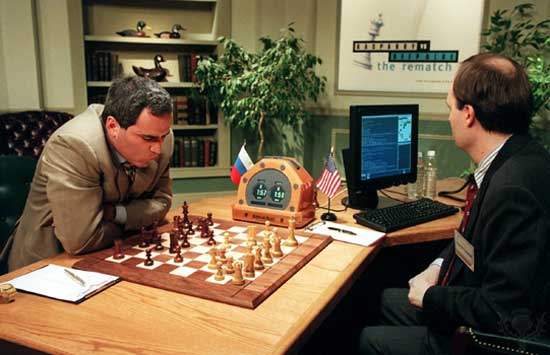
\includegraphics[height=5.5cm]{Diagrams/KasparovDeepBlue.jpg}
	\centering
\end{figure}
\end{frame}

\begin{frame}
\frametitle{Kasparov vs Deep Blue}
Great display of artifical intelligence \\
Techniques employed by IBM
\begin{itemize}
	\item Brute force deterministic approach
	\item human knowledge
\end{itemize}
Limitation
\begin{itemize}
	\item scalability into larger search spaces
\end{itemize}
Monte Carlo tree search (MCTS) is an alternative method
\end{frame}

\begin{frame}
  \frametitle{Outline}
  \tableofcontents[] 
\end{frame}

\begin{frame}
\frametitle{Monte Carlo Tree Search (MCTS)}
%cite british Go organisation http://www.britgo.org/learners/chessgo.html
\begin{itemize}
	\item Combines random sampling and game trees
	\item Probabilistic not deterministic
	\item Useful for problems with larger search spaces
\end{itemize}
\end{frame}

\begin{frame}
\frametitle{Two MCTS Applications}
Go
\begin{itemize}
	\item Board game about positional advantage
	\item Game board for Chess: 8x8
	\item Possible games of Chess: 10\textsuperscript{120}
	\item Game board for Go: 19x19
	\item Possible games of Go: 10\textsuperscript{761}
\end{itemize}
Narrative generation
\begin{itemize}
	\item Useful Applications
	\begin{itemize}
		\item Video game replay value
		\item educational applications
	\end{itemize}
	\item The search space scales with the number of characters, items, locations, and actions
\end{itemize}
\end{frame}

\section{Naive MCTS Implementation}

\begin{frame}
\frametitle{Outline}
\tableofcontents[currentsection]
\end{frame}

\begin{frame}[fragile]
\frametitle{TicTacToe Diagram}
\begin{figure}[h]
	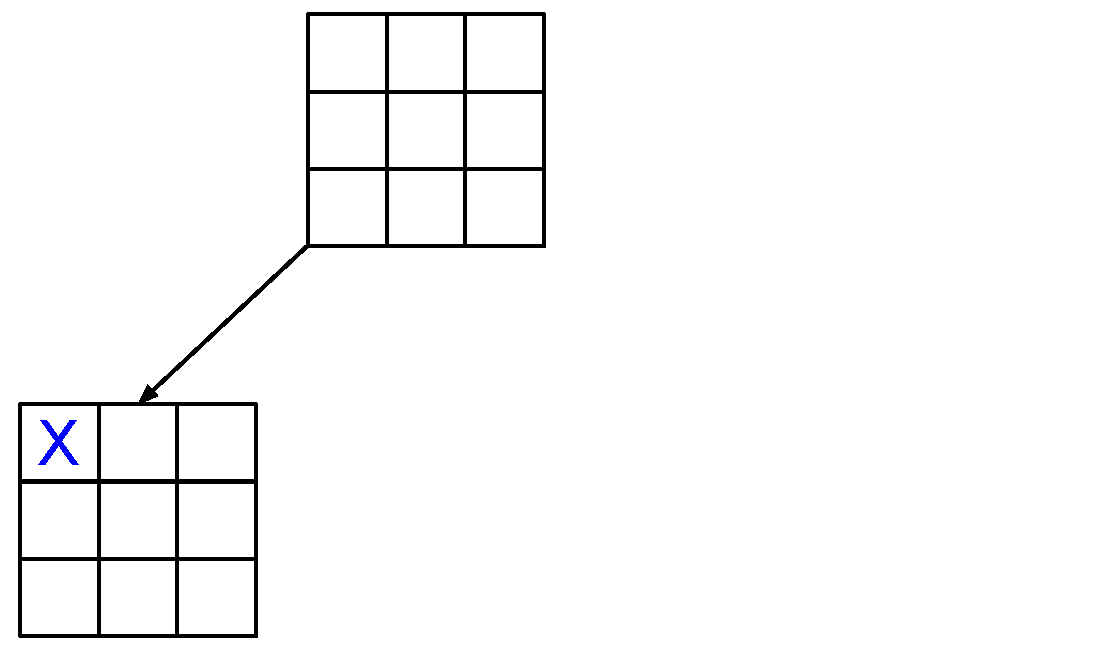
\includegraphics[width=8.5cm]{Diagrams/TicTacToe/TicTacToeTreeOne.pdf}
	\centering
\end{figure}
\end{frame}

\begin{frame}[fragile]
\frametitle{TicTacToe Diagram}
\begin{figure}[h]
	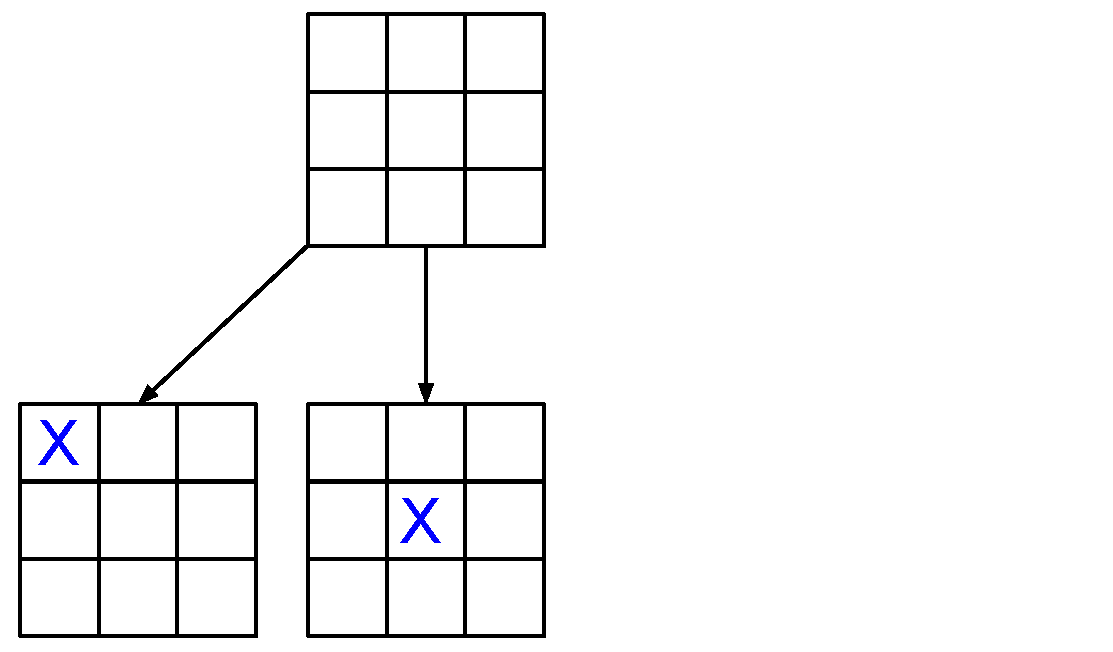
\includegraphics[width=8.5cm]{Diagrams/TicTacToe/TicTacToeTreeTwo.pdf}
	\centering
\end{figure}
\end{frame}

\begin{frame}[fragile]
\frametitle{TicTacToe Diagram}
\begin{figure}[h]
	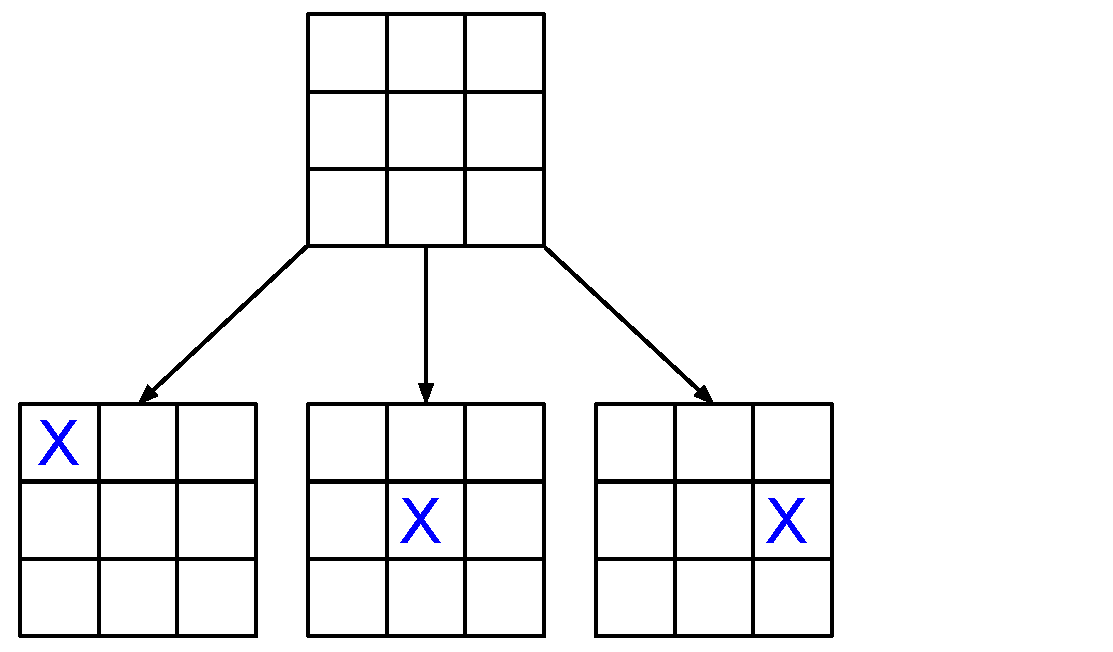
\includegraphics[width=8.5cm]{Diagrams/TicTacToe/TicTacToeTreeThree.pdf}
	\centering
\end{figure}
\end{frame}

\begin{frame}[fragile]
\frametitle{TicTacToe Diagram More Levels}
\begin{figure}[h]
	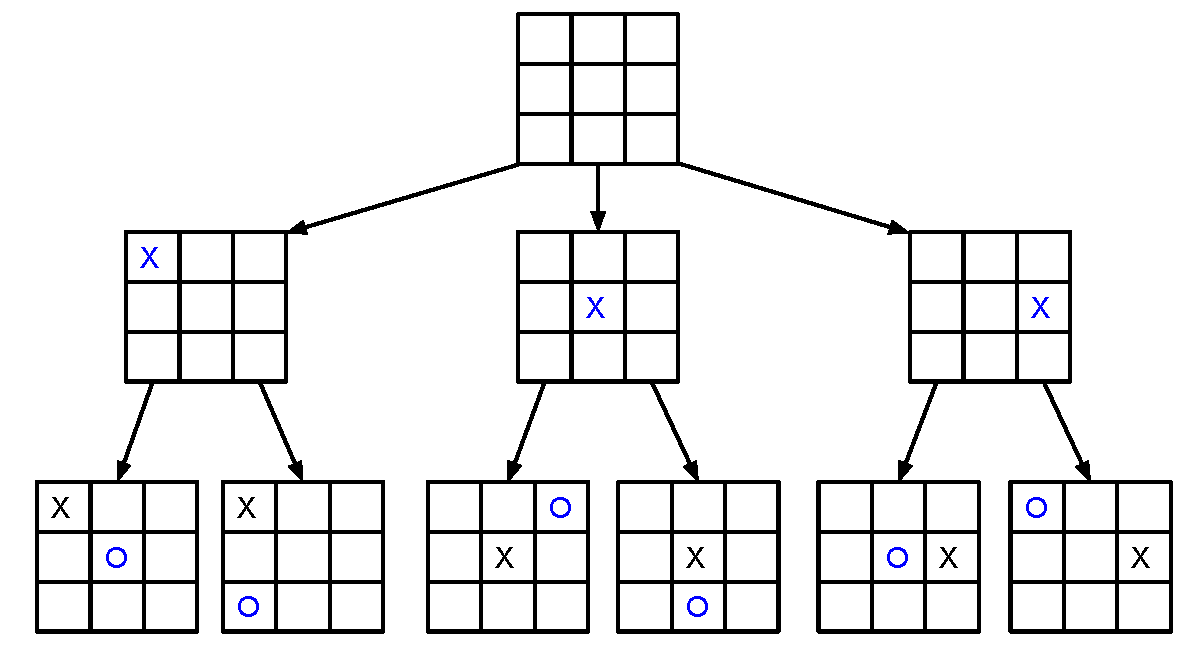
\includegraphics[width=8.5cm]{Diagrams/TicTacToe/TicTacToeTreeMultiLevel.pdf}
	\centering
\end{figure}
\end{frame}

\begin{frame}[fragile]
\frametitle{TicTacToe Diagram}
\begin{figure}[h]
	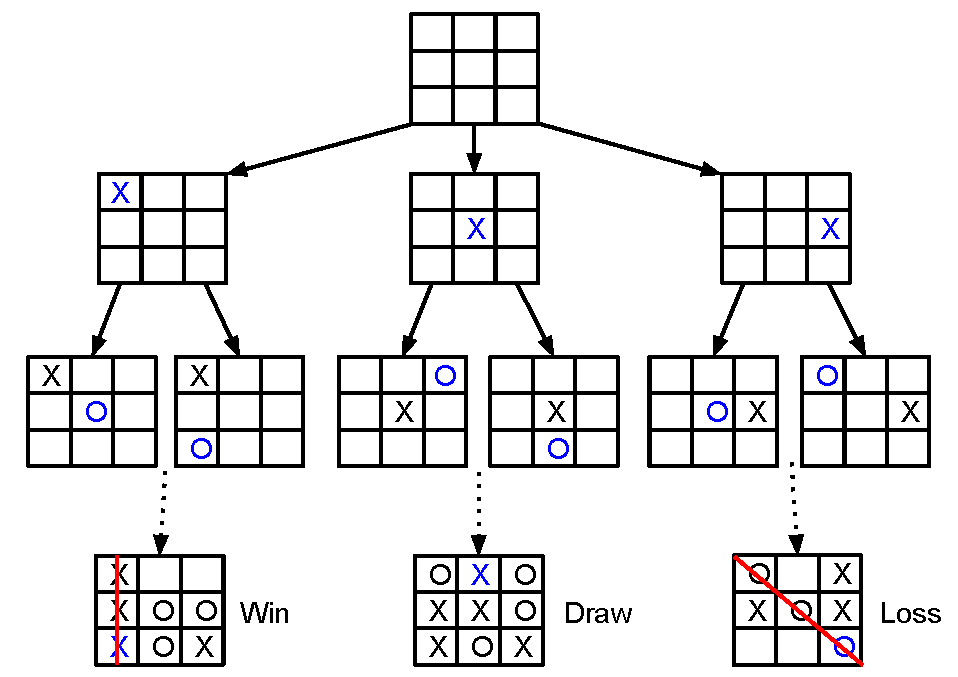
\includegraphics[width=8.5cm]{Diagrams/TicTacToe/TicTacToeTreeExtended.pdf}
	\centering
\end{figure}
\end{frame}

\begin{frame}[fragile]
\frametitle{TicTacToe Diagram}
\begin{figure}[h]
	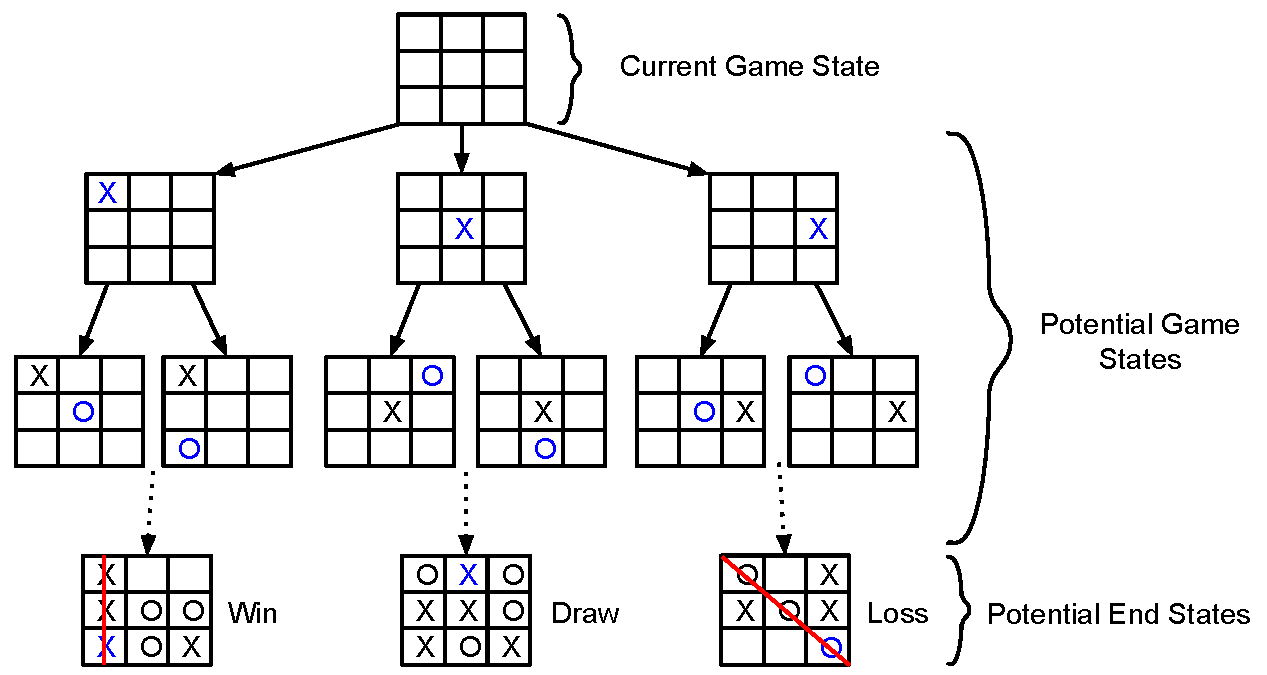
\includegraphics[width=10cm]{Diagrams/TicTacToe/TicTacToeTreeExtendedLabeled.pdf}
	\centering
\end{figure}
\end{frame}

\begin{frame}[fragile]
\frametitle{Tree Structure}
\begin{figure}[h]
	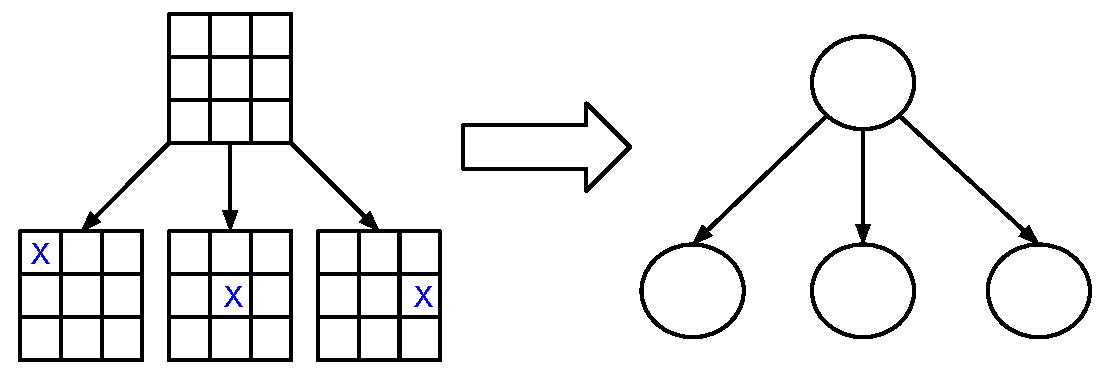
\includegraphics[width=10cm]{Diagrams/TicTacToe/MapToTree.pdf}
	\centering
\end{figure}
\end{frame}

\begin{frame}[fragile]
\frametitle{Sampling}
\begin{figure}[h]
	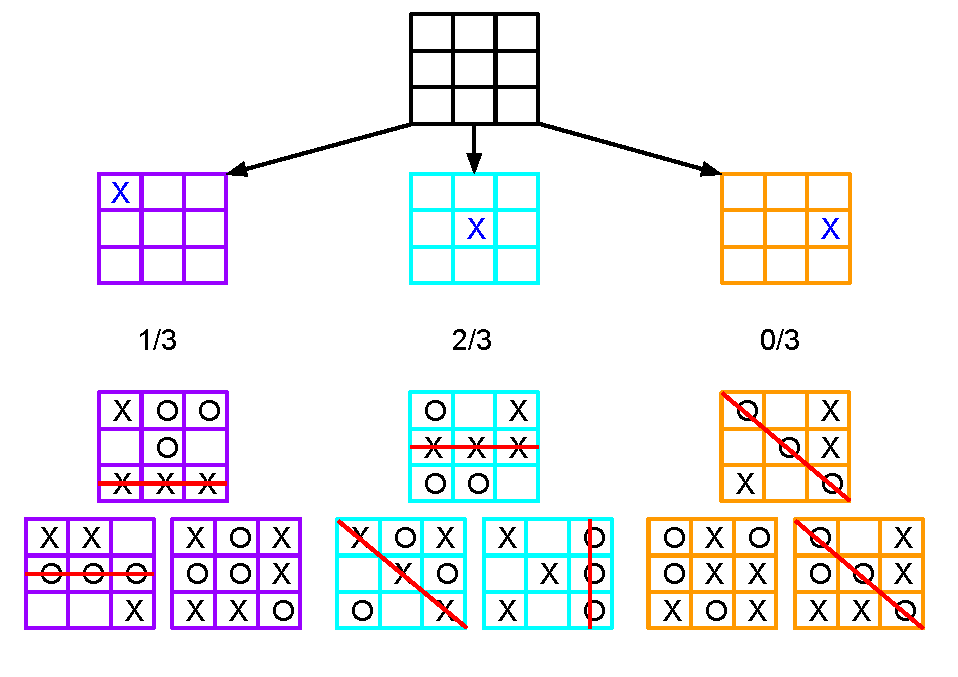
\includegraphics[width=8.5cm]{Diagrams/TicTacToe/TicTacToeTreeSampling.pdf}
	\centering
\end{figure}
\end{frame}

%%%%%%%%%%%%%%%Four Step full diagram begins%%%%%%%%%%%%%%%%%%%%%%%%%%%%

\begin{frame}[fragile]
\frametitle{Four Steps Diagram}
\begin{figure}[h]
	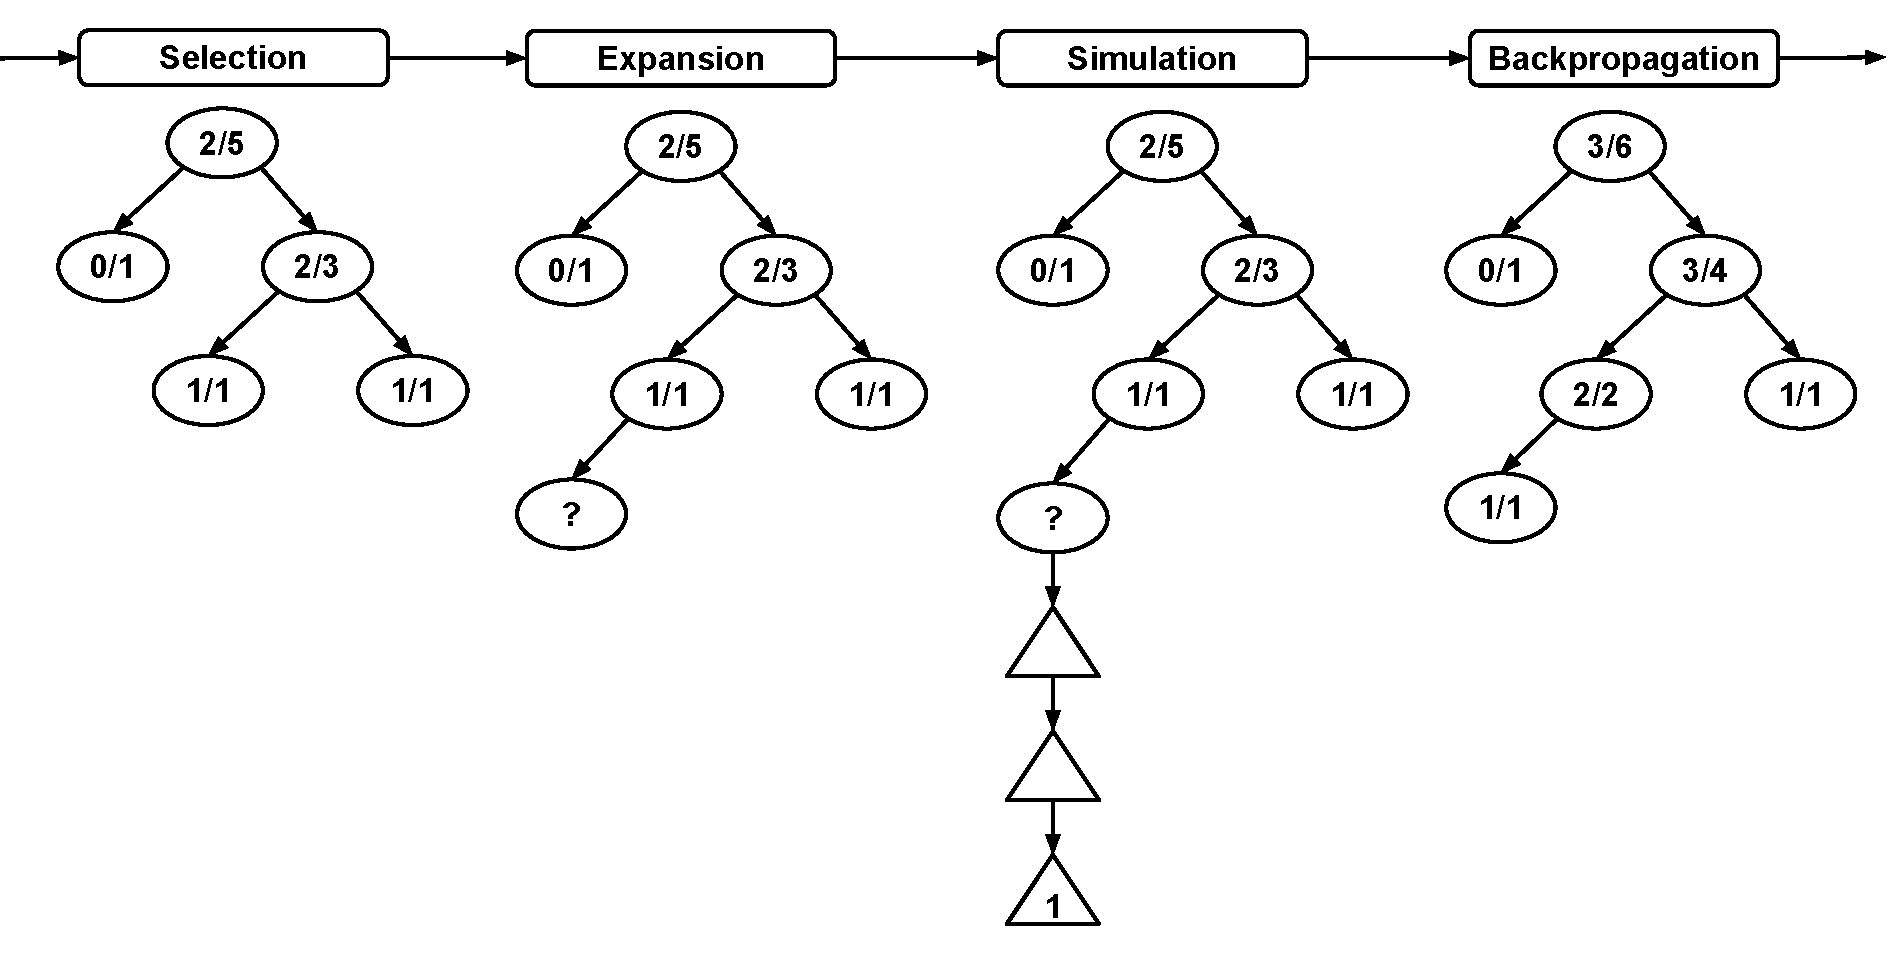
\includegraphics[width=11cm]{Diagrams/FourSteps/MCTSFourStepProcessWhole.pdf}
	\centering
\end{figure}
\end{frame}

\begin{frame}[fragile]
\frametitle{Four Steps Diagram}
\begin{figure}[h]
	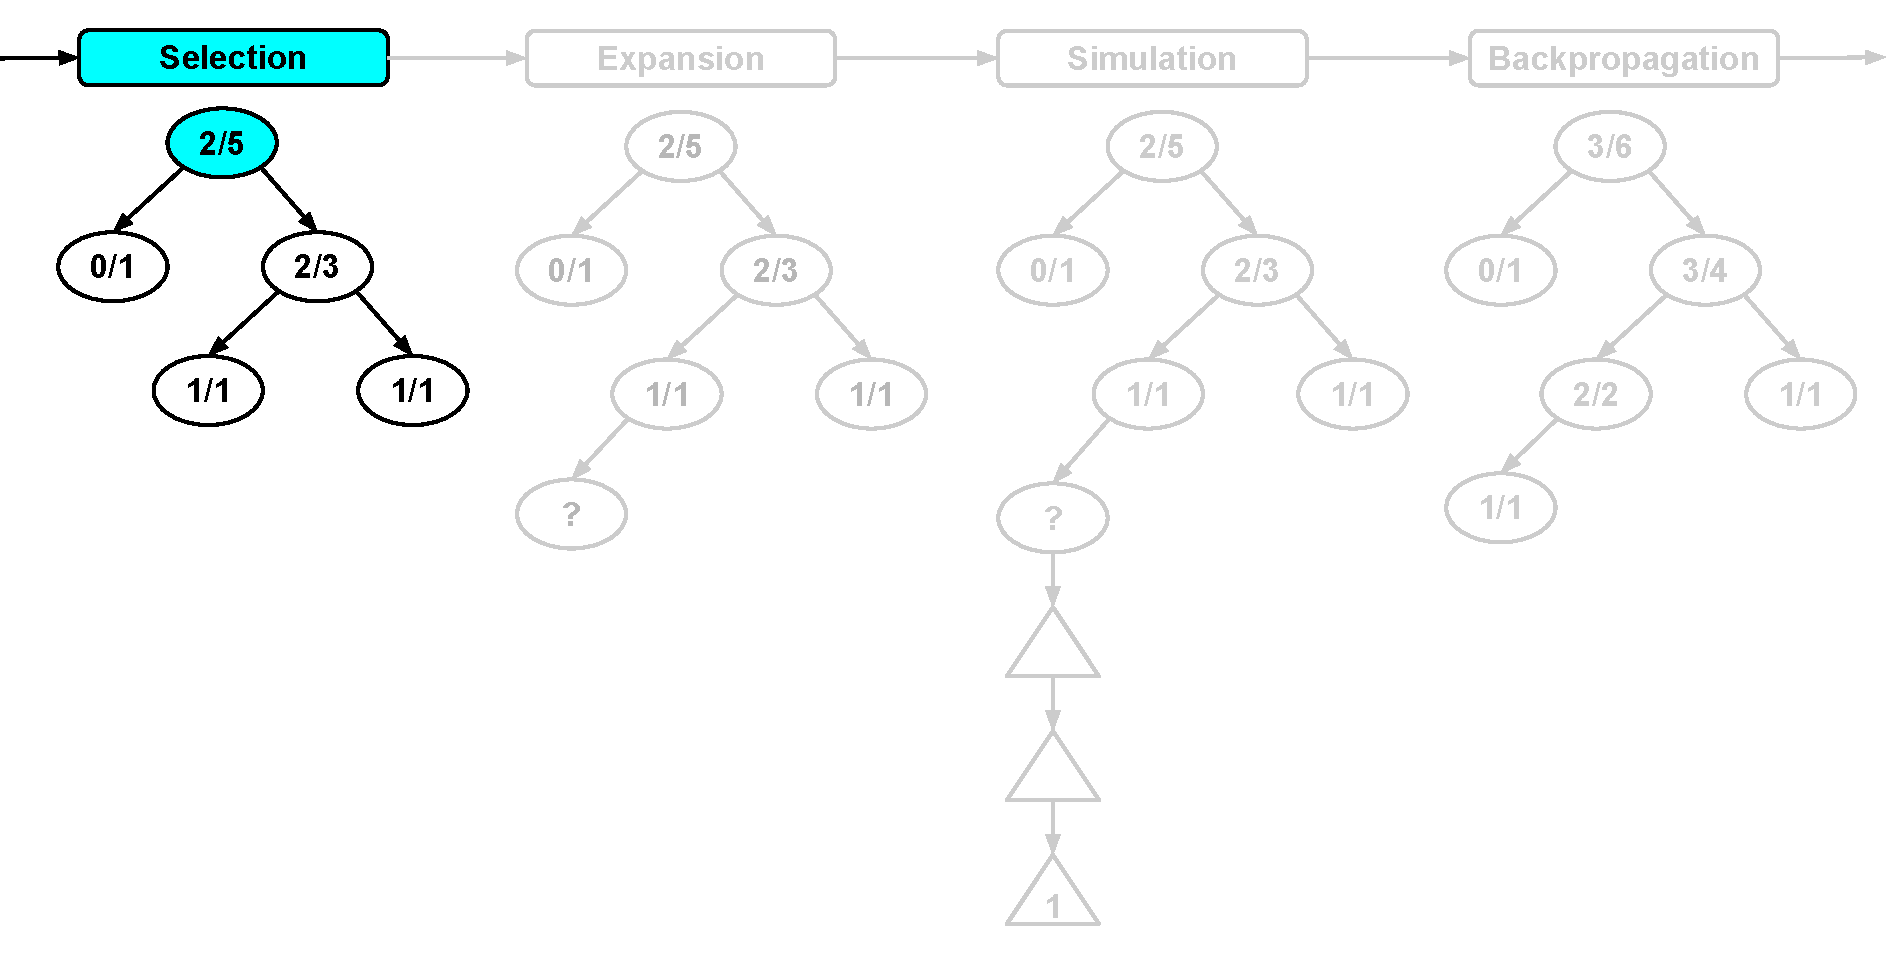
\includegraphics[width=11cm]{Diagrams/FourSteps/MCTSFourStepProcessOneOne.pdf}
	\centering
\end{figure}
\end{frame}

\begin{frame}[fragile]
\frametitle{Four Steps Diagram}
\begin{figure}[h]
	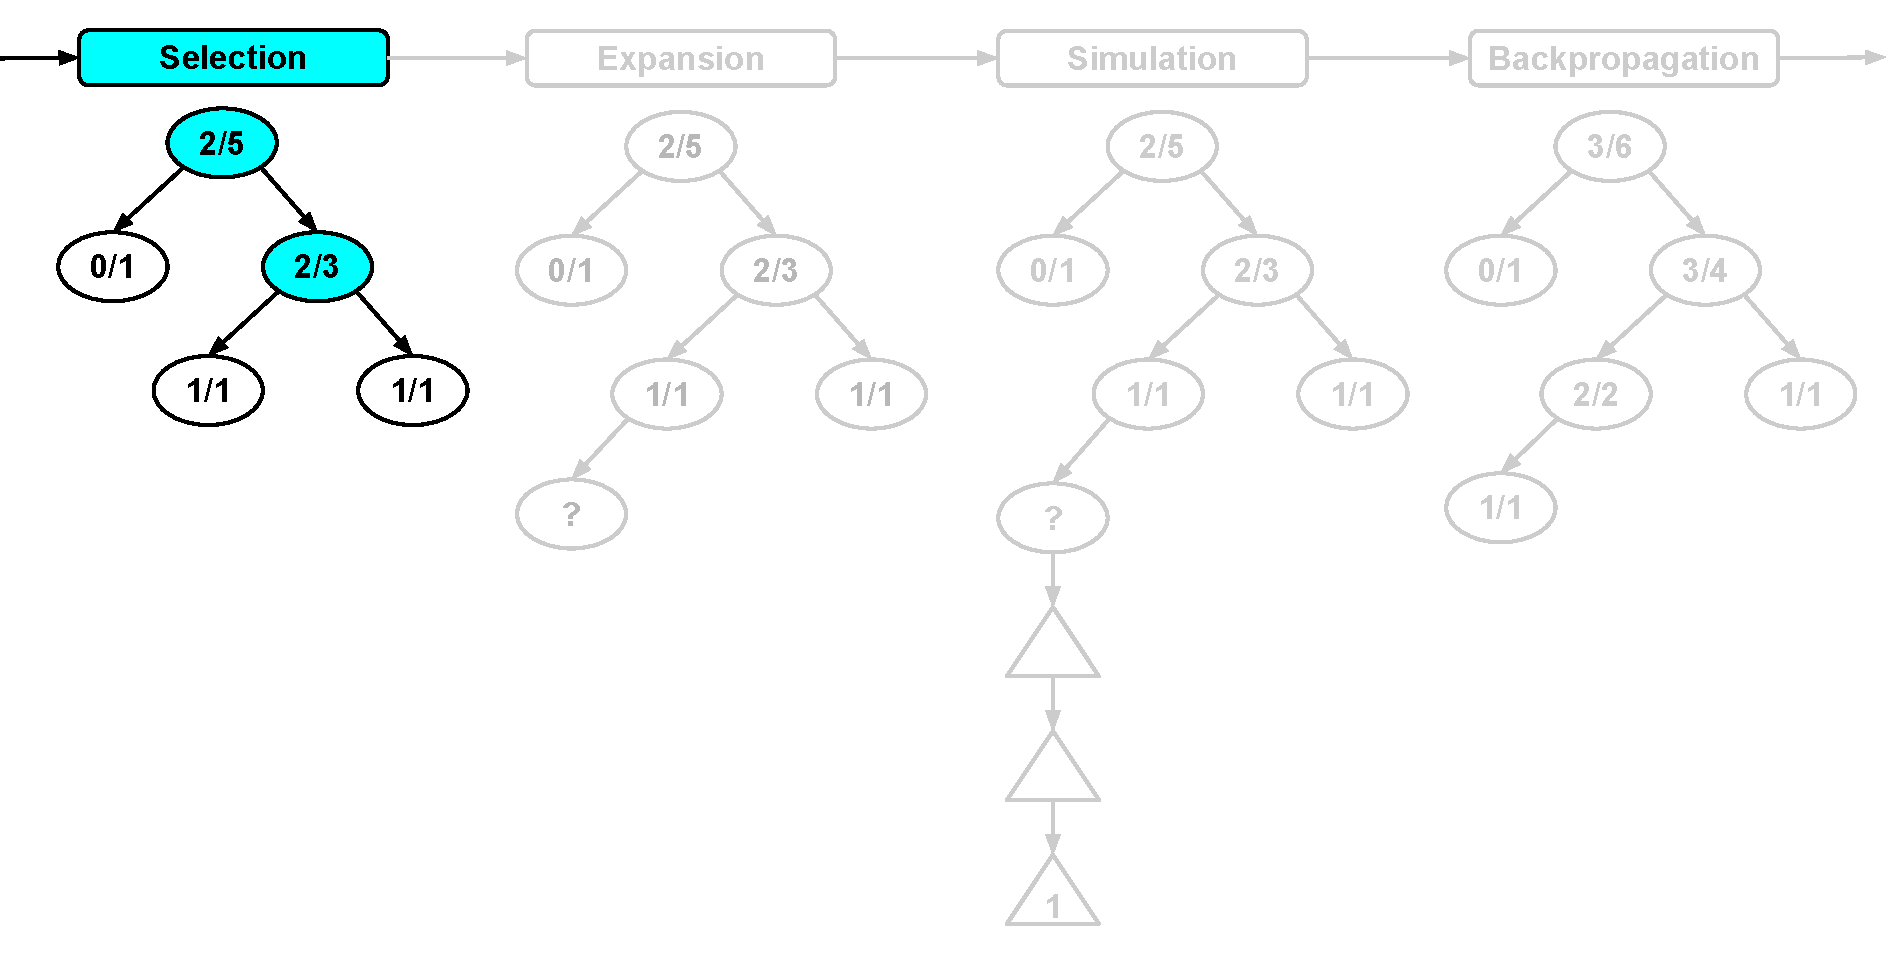
\includegraphics[width=11cm]{Diagrams/FourSteps/MCTSFourStepProcessOneTwo.pdf}
	\centering
\end{figure}
\end{frame}

\begin{frame}[fragile]
\frametitle{Four Steps Diagram}
\begin{figure}[h]
	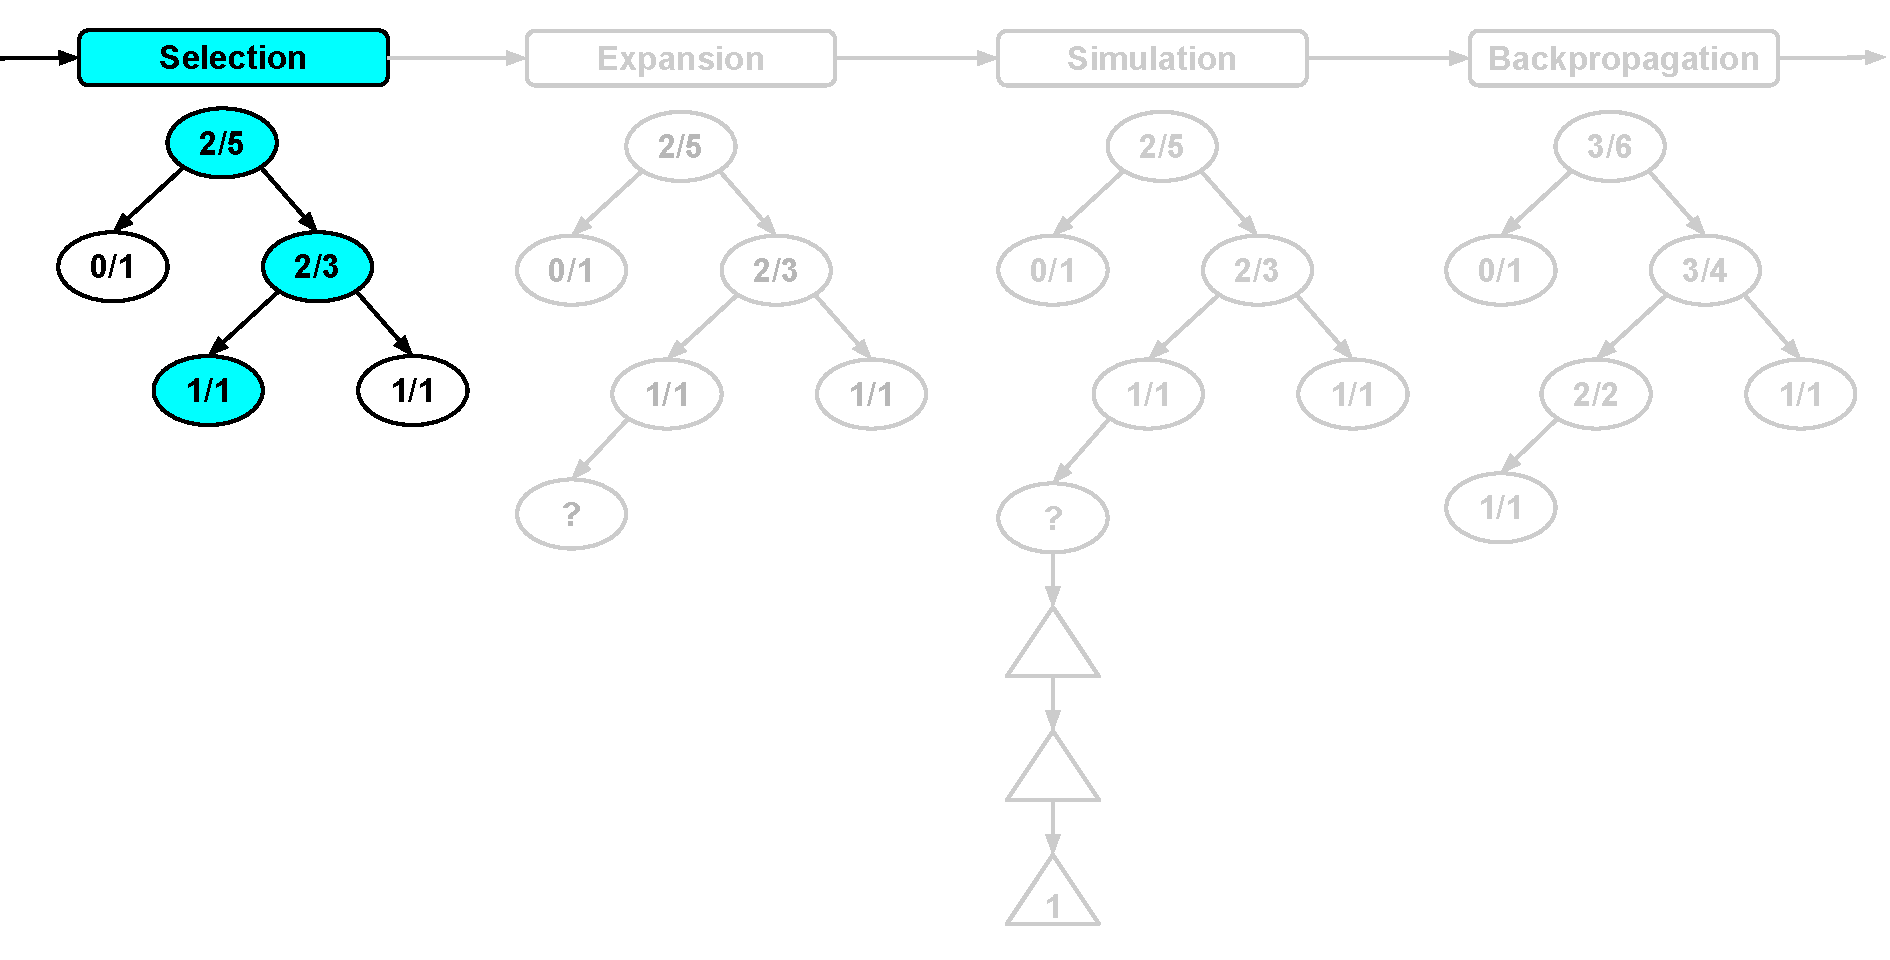
\includegraphics[width=11cm]{Diagrams/FourSteps/MCTSFourStepProcessOneThree.pdf}
	\centering
\end{figure}
\end{frame}

\begin{frame}[fragile]
\frametitle{Four Steps Diagram}
\begin{figure}[h]
	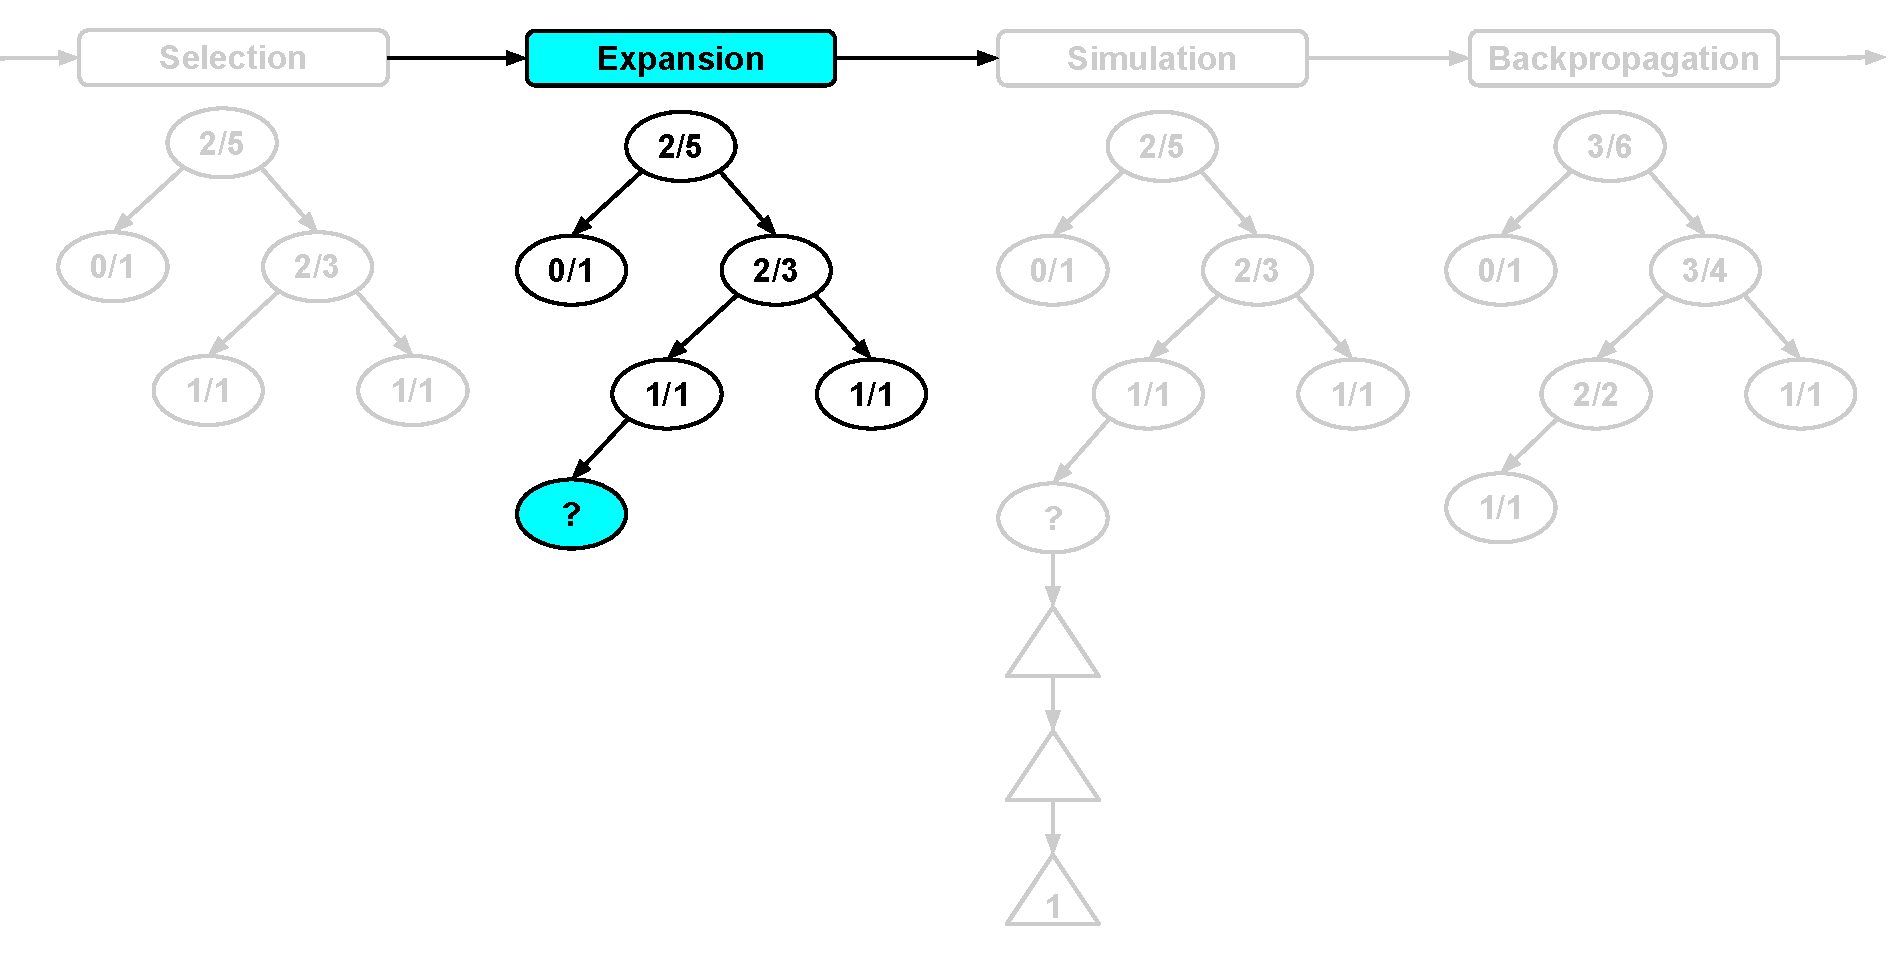
\includegraphics[width=11cm]{Diagrams/FourSteps/MCTSFourStepProcessTwo.pdf}
	\centering
\end{figure}
\end{frame}

\begin{frame}[fragile]
\frametitle{Four Steps Diagram}
\begin{figure}[h]
	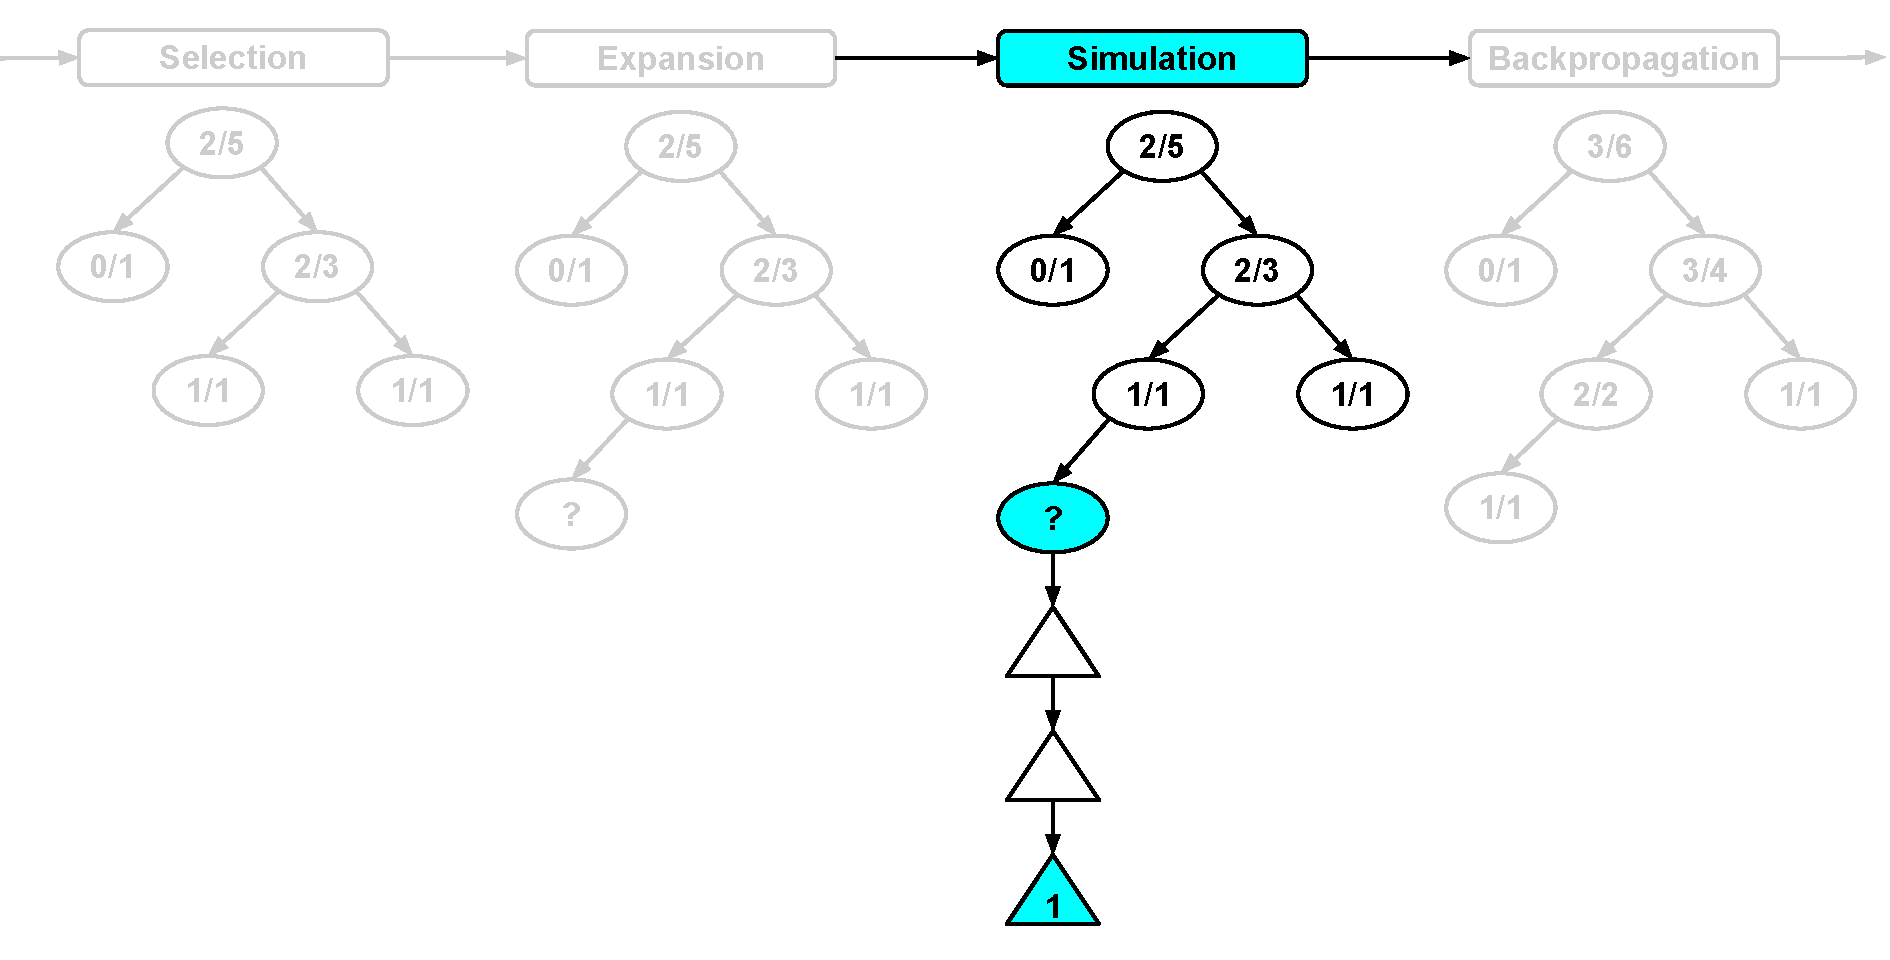
\includegraphics[width=11cm]{Diagrams/FourSteps/MCTSFourStepProcessThree.pdf}
	\centering
\end{figure}
\end{frame}

\begin{frame}[fragile]
\frametitle{Four Steps Diagram}
\begin{figure}[h]
	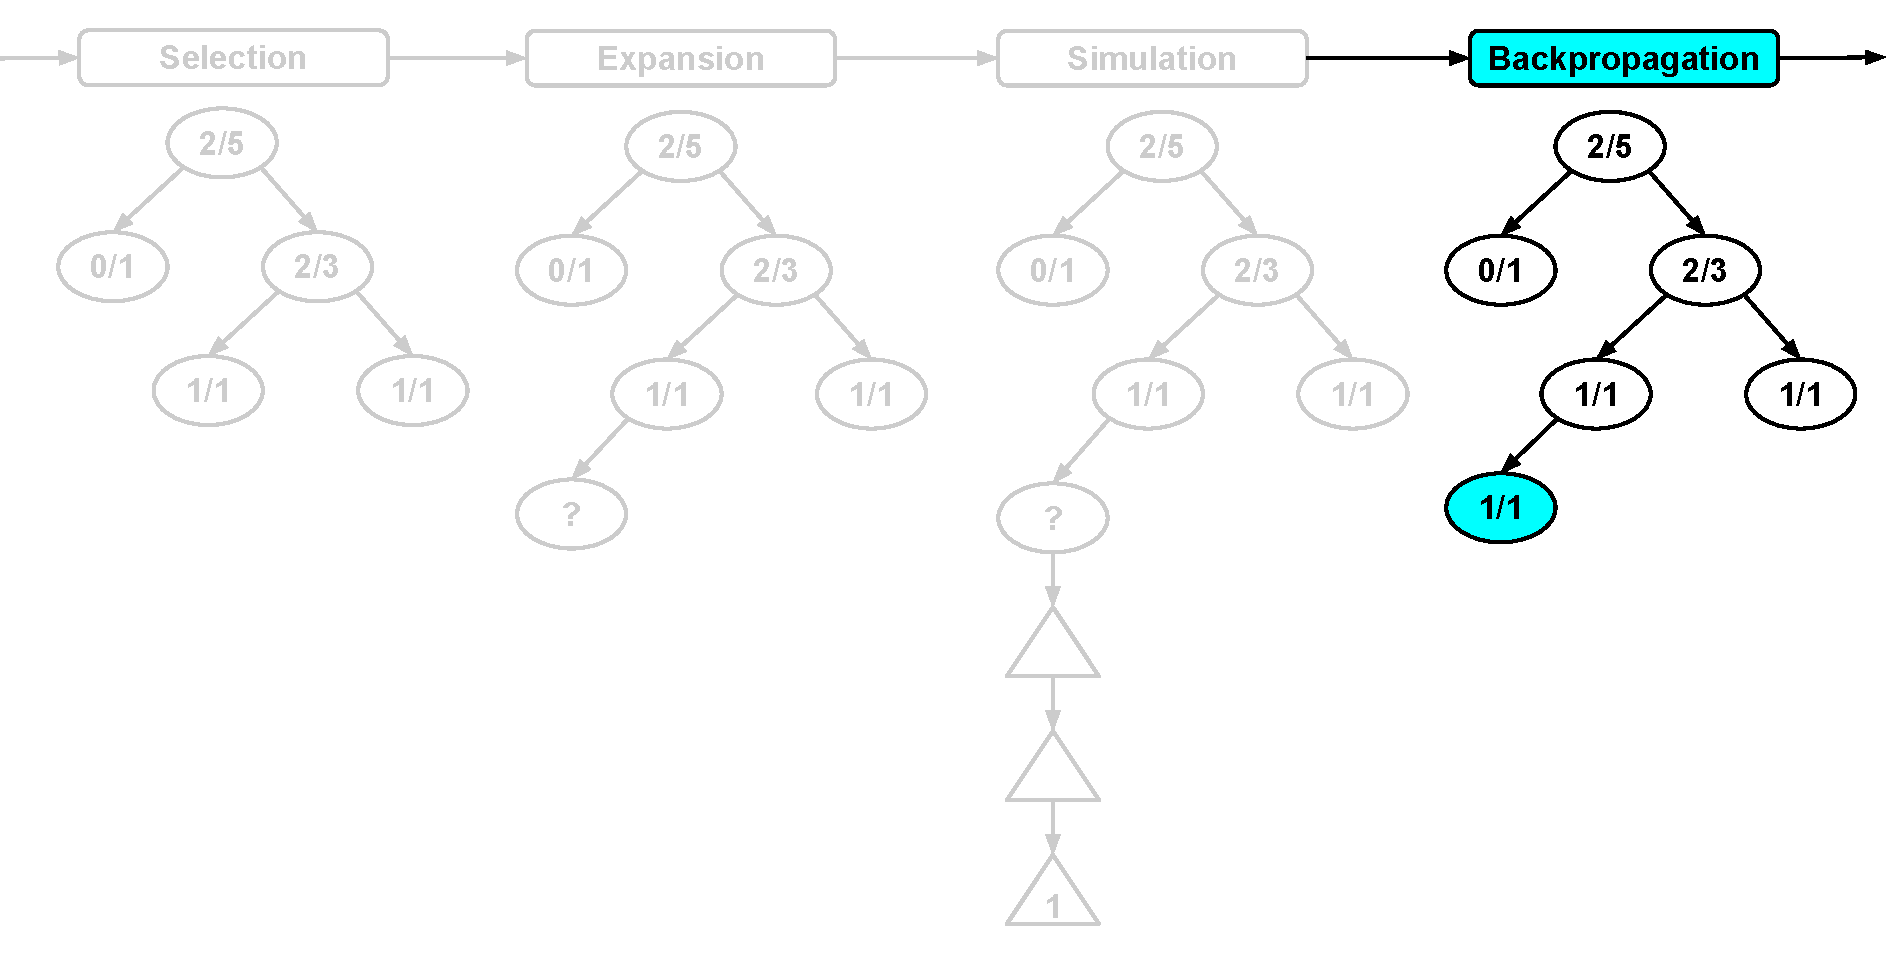
\includegraphics[width=11cm]{Diagrams/FourSteps/MCTSFourStepProcessFourOne.pdf}
	\centering
\end{figure}
\end{frame}

\begin{frame}[fragile]
\frametitle{Four Steps Diagram}
\begin{figure}[h]
	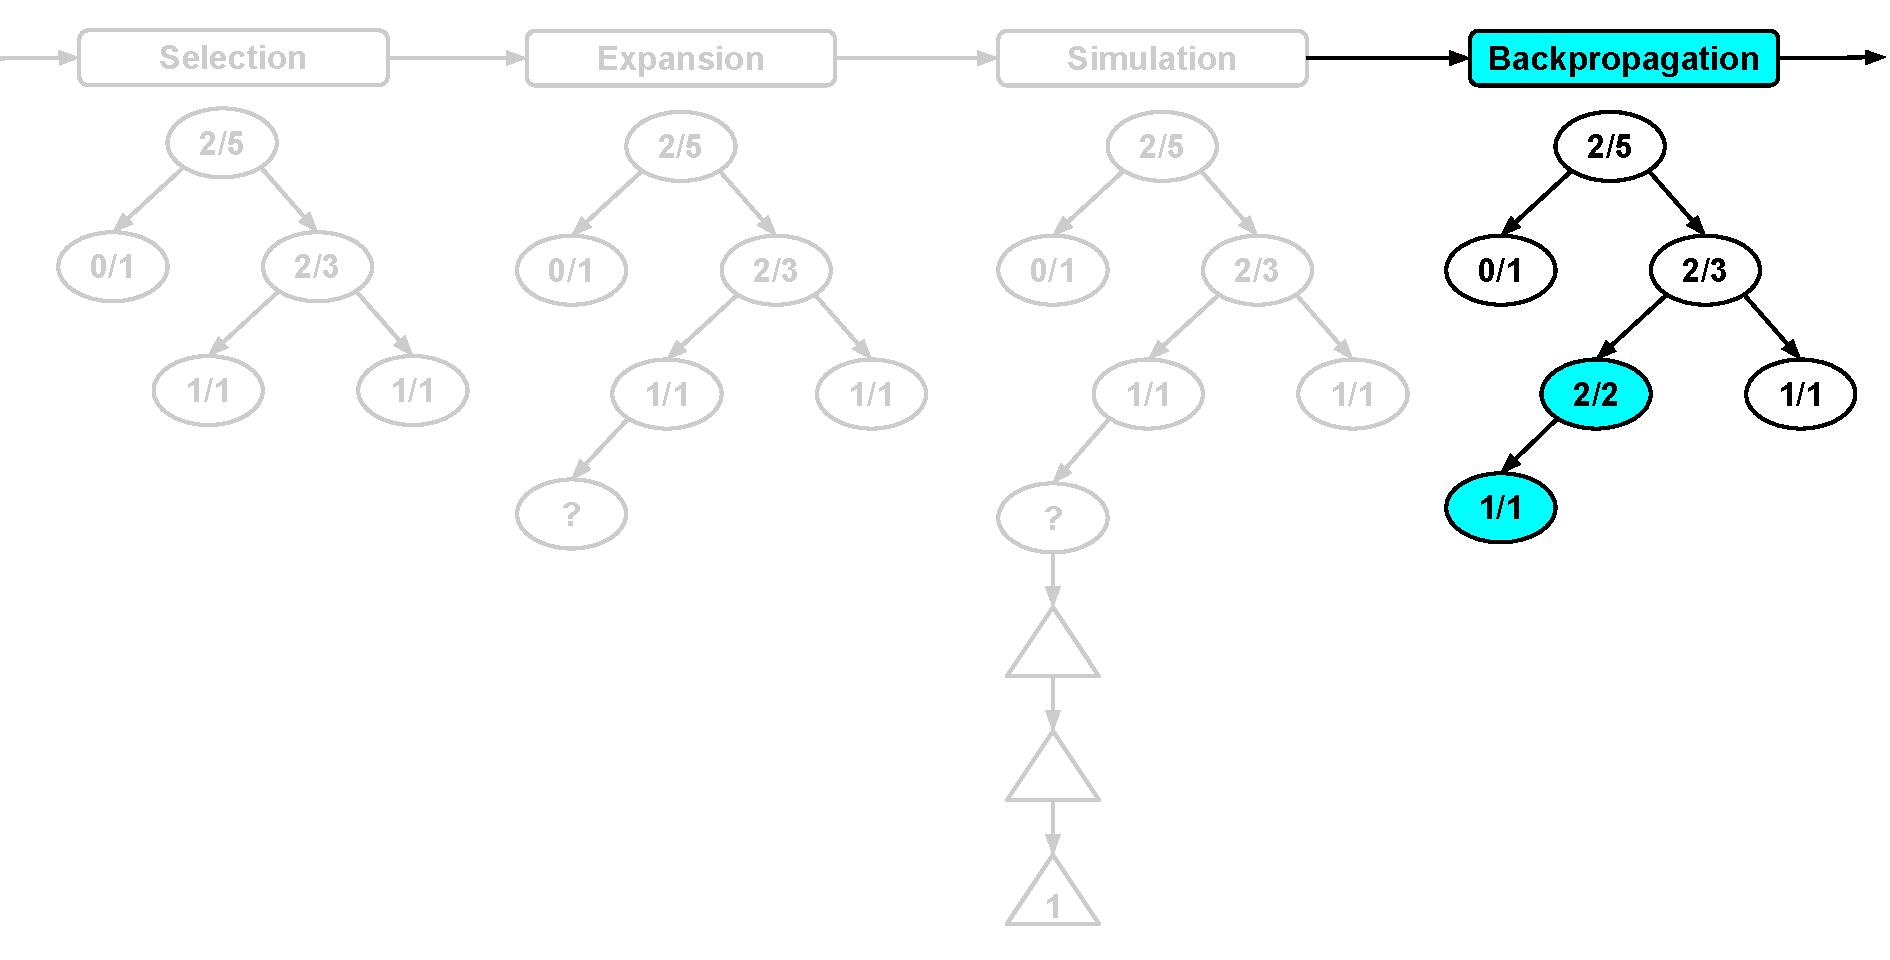
\includegraphics[width=11cm]{Diagrams/FourSteps/MCTSFourStepProcessFourTwo.pdf}
	\centering
\end{figure}
\end{frame}

\begin{frame}[fragile]
\frametitle{Four Steps Diagram}
\begin{figure}[h]
	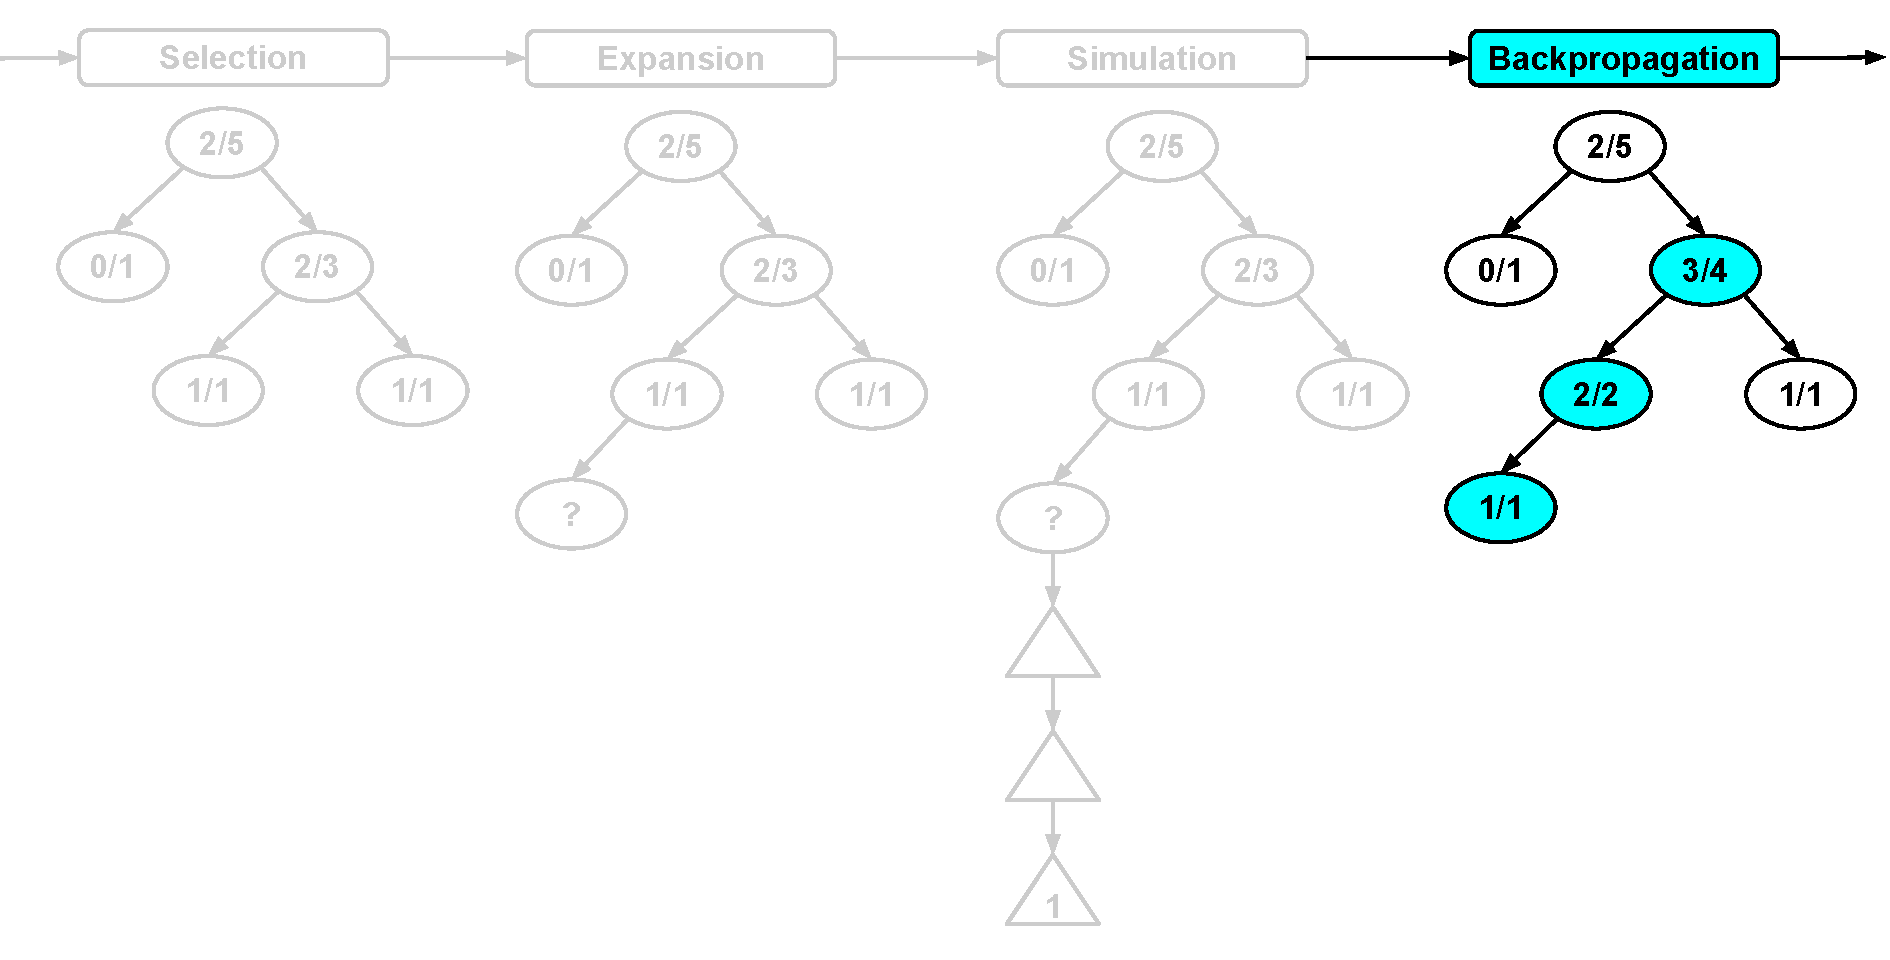
\includegraphics[width=11cm]{Diagrams/FourSteps/MCTSFourStepProcessFourThree.pdf}
	\centering
\end{figure}
\end{frame}

\begin{frame}[fragile]
\frametitle{Four Steps Diagram}
\begin{figure}[h]
	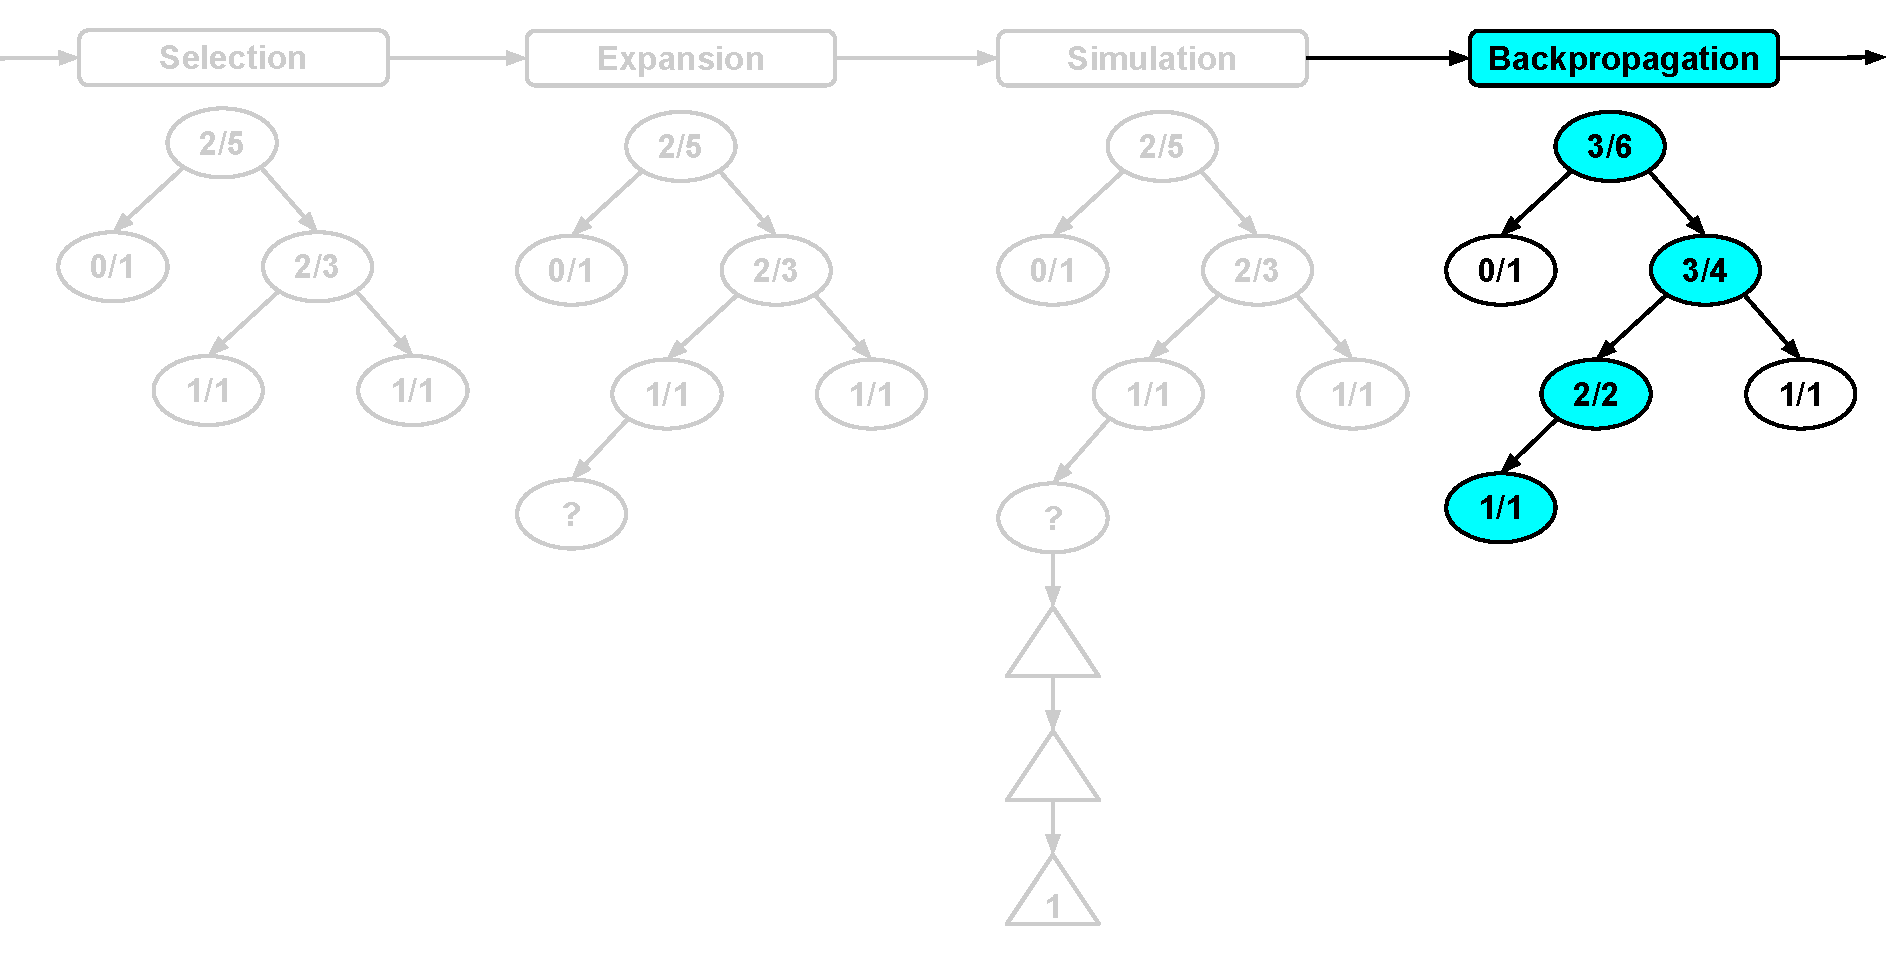
\includegraphics[width=11cm]{Diagrams/FourSteps/MCTSFourStepProcessFourFour.pdf}
	\centering
\end{figure}
\end{frame}

\begin{frame}[fragile]
\frametitle{Four Steps Diagram}
\begin{figure}[h]
	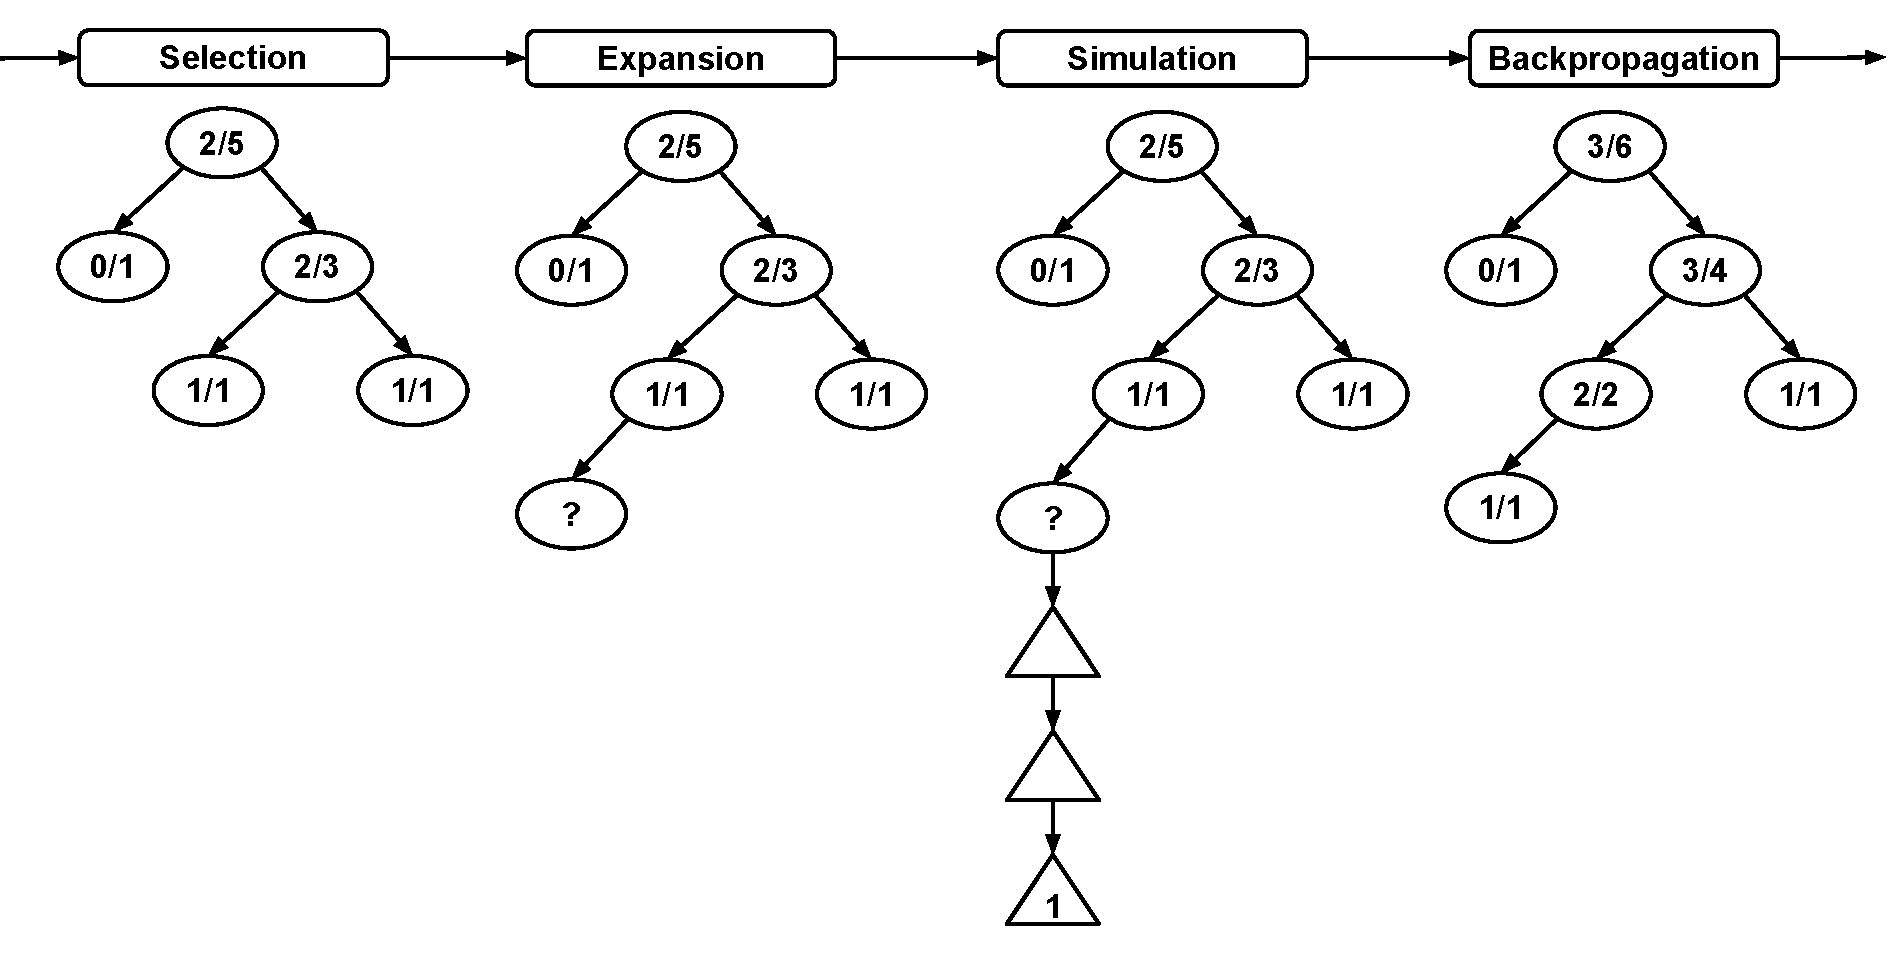
\includegraphics[width=11cm]{Diagrams/FourSteps/MCTSFourStepProcessWhole.pdf}
	\centering
\end{figure}
\end{frame}

%%%%%%%%%%%%%%%%%%%%%%%%%Four Step diagram ends%%%%%%%%%%%%%%%%%%%%%%%%%%%%%%%%

%%%%%%%%%%%%%%%%%%%%%%%%%First example walkthrough%%%%%%%%%%%%%%%%%%%%%%%%%%%%%%

\begin{frame}[fragile]
\frametitle{Four Steps Diagram}
\begin{figure}[h]
	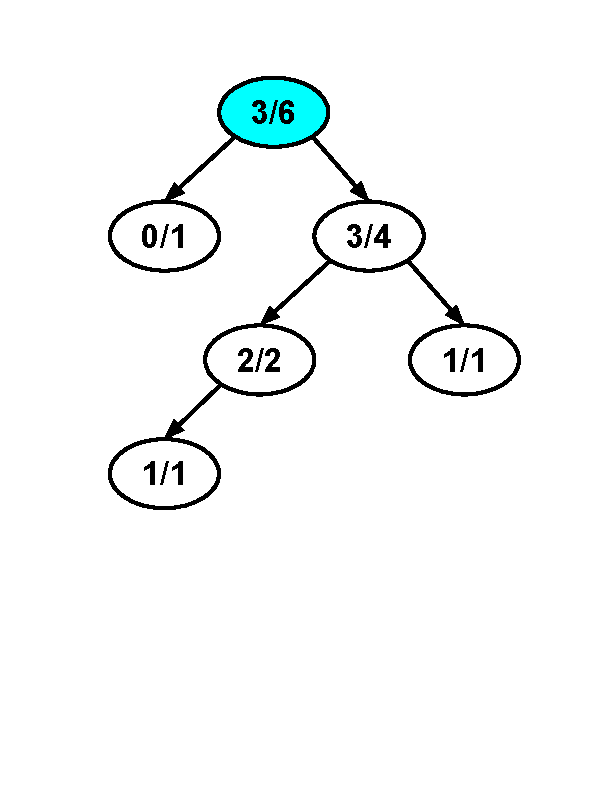
\includegraphics[width=6.5cm]{Diagrams/MCTSShort/MCTSShortOneOneOne.pdf}
	\centering
\end{figure}
\end{frame}


\begin{frame}[fragile]
\frametitle{Four Steps Diagram}
\begin{figure}[h]
	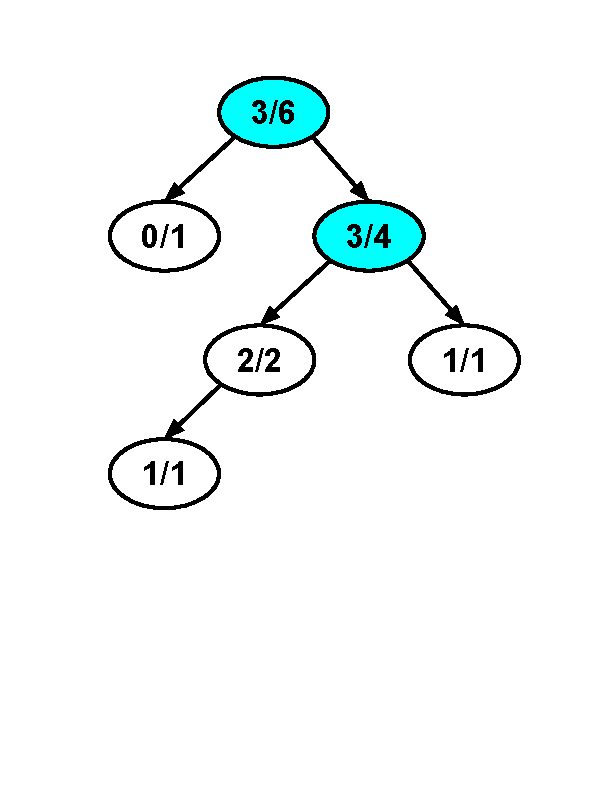
\includegraphics[width=6.5cm]{Diagrams/MCTSShort/MCTSShortOneOneTwo.pdf}
	\centering
\end{figure}
\end{frame}


\begin{frame}[fragile]
\frametitle{Four Steps Diagram}
\begin{figure}[h]
	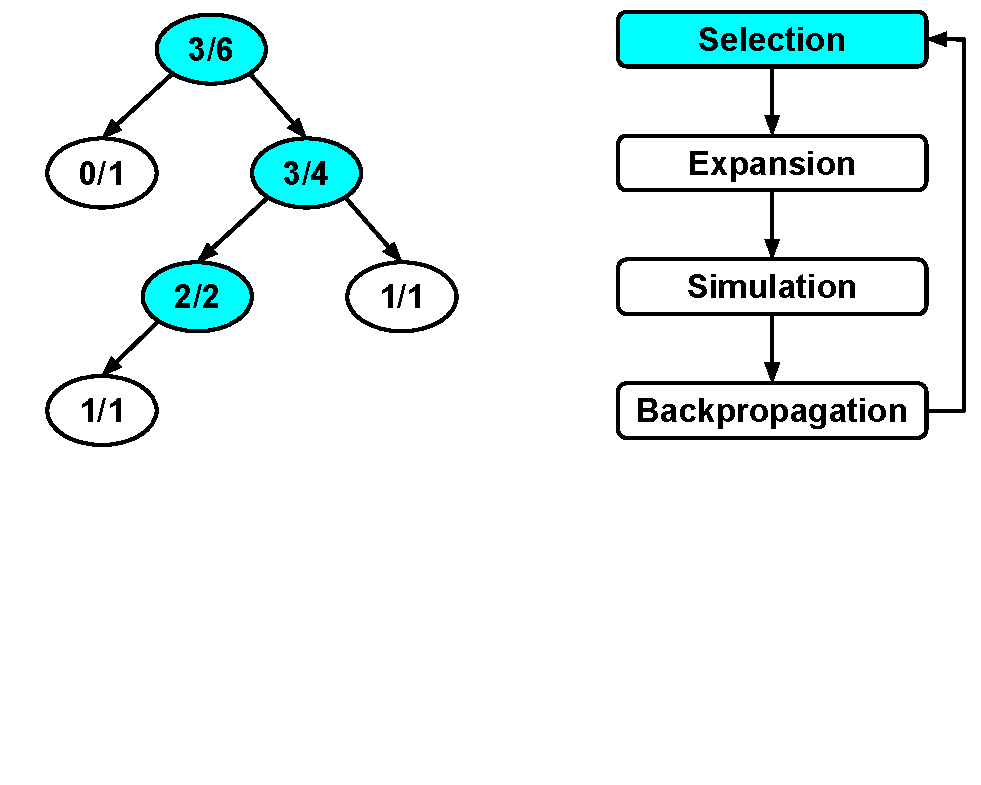
\includegraphics[width=6.5cm]{Diagrams/MCTSShort/MCTSShortOneOneThree.pdf}
	\centering
\end{figure}
\end{frame}


\begin{frame}[fragile]
\frametitle{Four Steps Diagram}
\begin{figure}[h]
	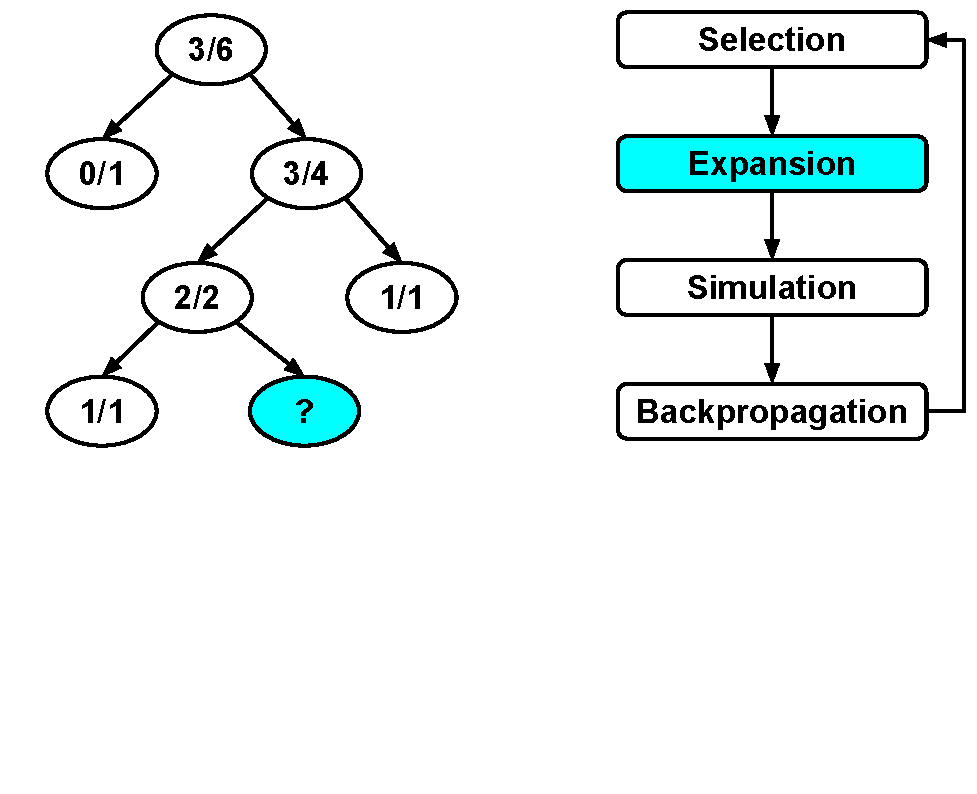
\includegraphics[width=6.5cm]{Diagrams/MCTSShort/MCTSShortOneTwo.pdf}
	\centering
\end{figure}
\end{frame}

\begin{frame}[fragile]
\frametitle{Four Steps Diagram}
\begin{figure}[h]
	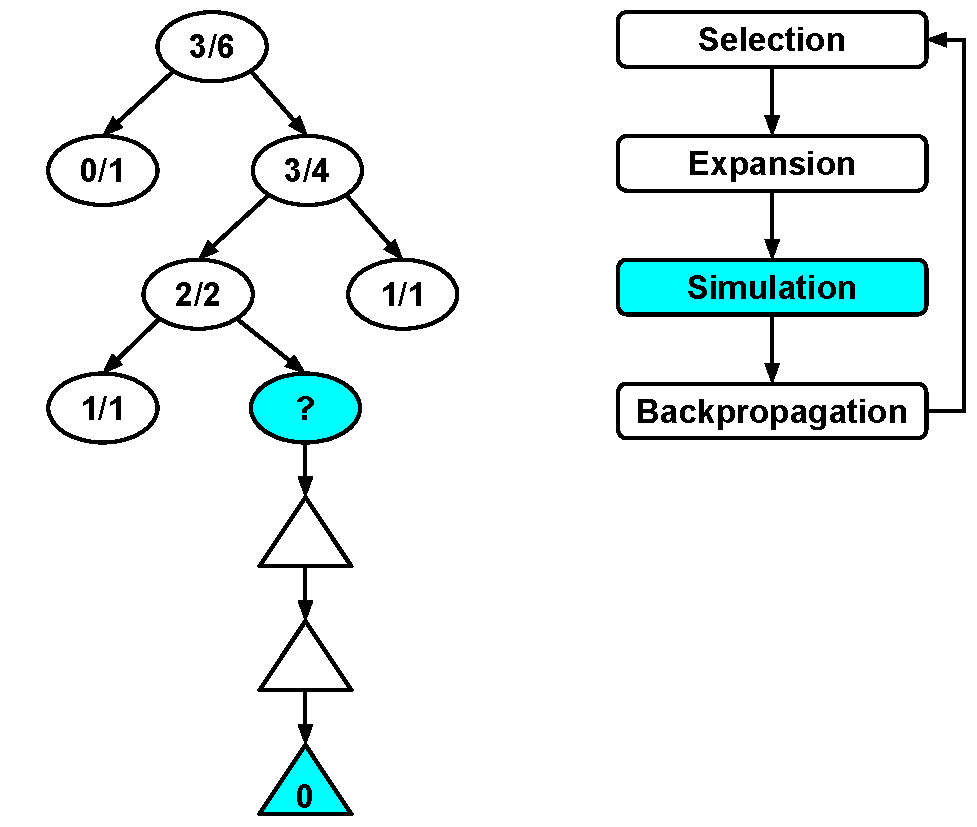
\includegraphics[width=6.5cm]{Diagrams/MCTSShort/MCTSShortOneThree.pdf}
	\centering
\end{figure}
\end{frame}

\begin{frame}[fragile]
\frametitle{Four Steps Diagram}
\begin{figure}[h]
	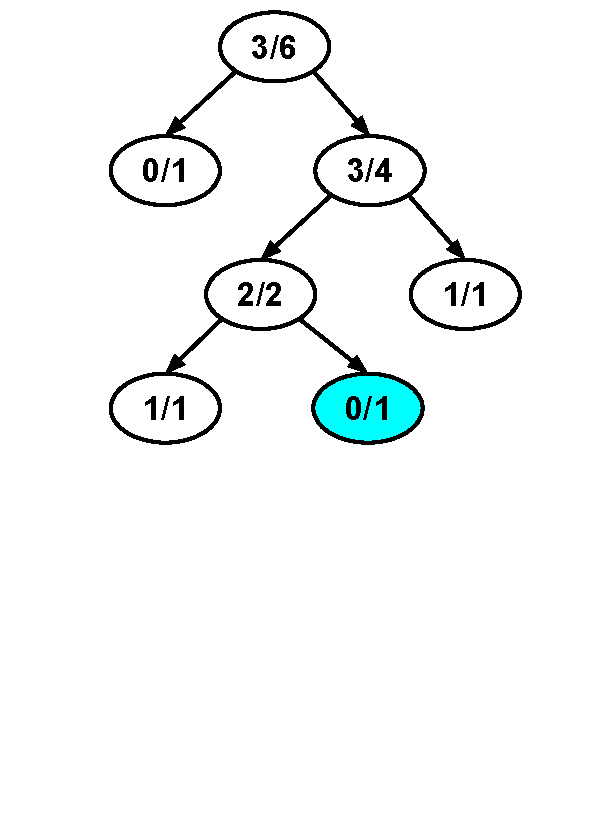
\includegraphics[width=6.5cm]{Diagrams/MCTSShort/MCTSShortOneFourOne.pdf}
	\centering
\end{figure}
\end{frame}

\begin{frame}[fragile]
\frametitle{Four Steps Diagram}
\begin{figure}[h]
	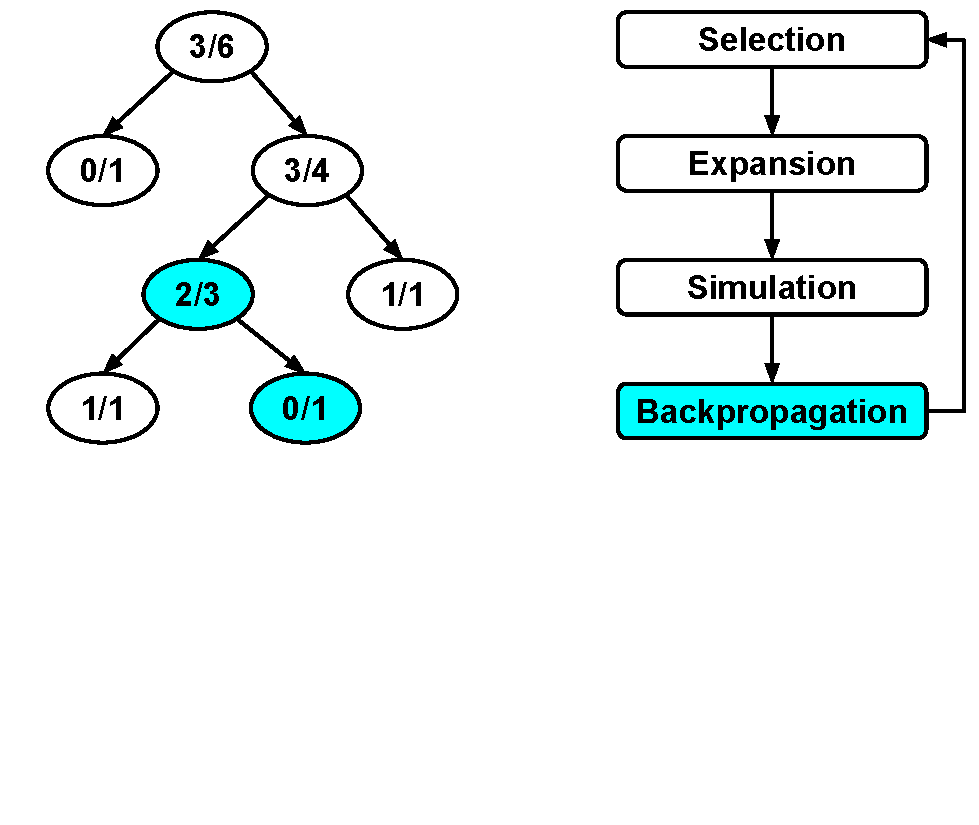
\includegraphics[width=6.5cm]{Diagrams/MCTSShort/MCTSShortOneFourTwo.pdf}
	\centering
\end{figure}
\end{frame}

\begin{frame}[fragile]
\frametitle{Four Steps Diagram}
\begin{figure}[h]
	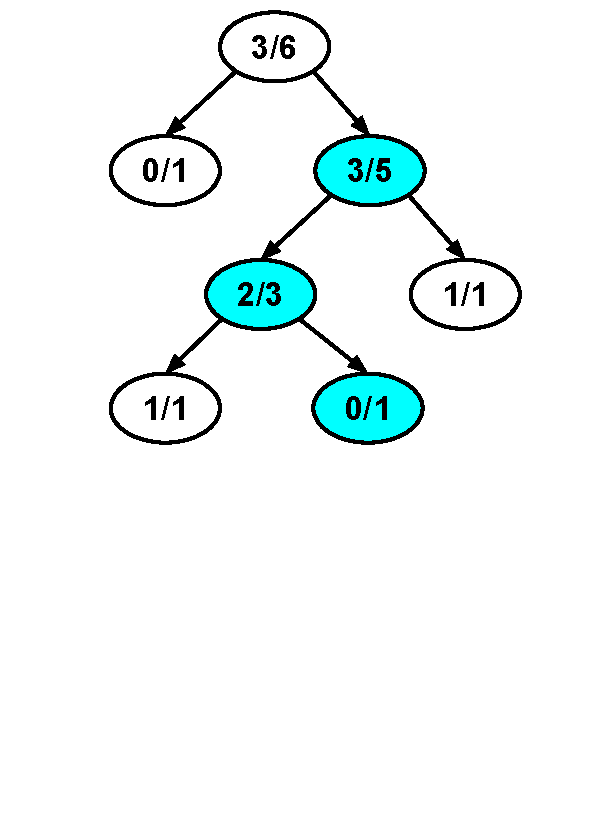
\includegraphics[width=6.5cm]{Diagrams/MCTSShort/MCTSShortOneFourThree.pdf}
	\centering
\end{figure}
\end{frame}

\begin{frame}[fragile]
\frametitle{Four Steps Diagram}
\begin{figure}[h]
	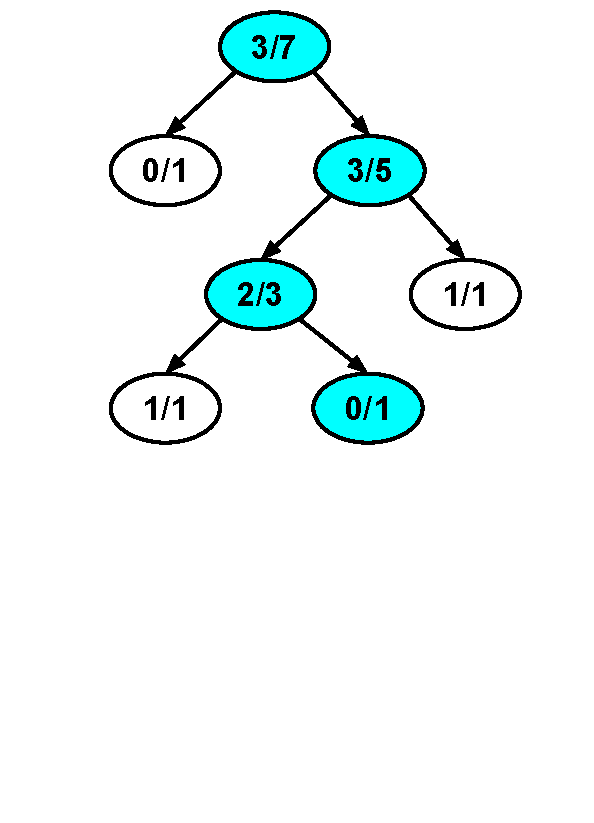
\includegraphics[width=6.5cm]{Diagrams/MCTSShort/MCTSShortOneFourFour.pdf}
	\centering
\end{figure}
\end{frame}

%%%%%%%%%%%%%%%%%%%%%%%%Second example walkthrough%%%%%%%%%%%%%%%%%%%%%%%%%%%%%%%

\begin{frame}[fragile]
\frametitle{Four Steps Diagram}
\begin{figure}[h]
	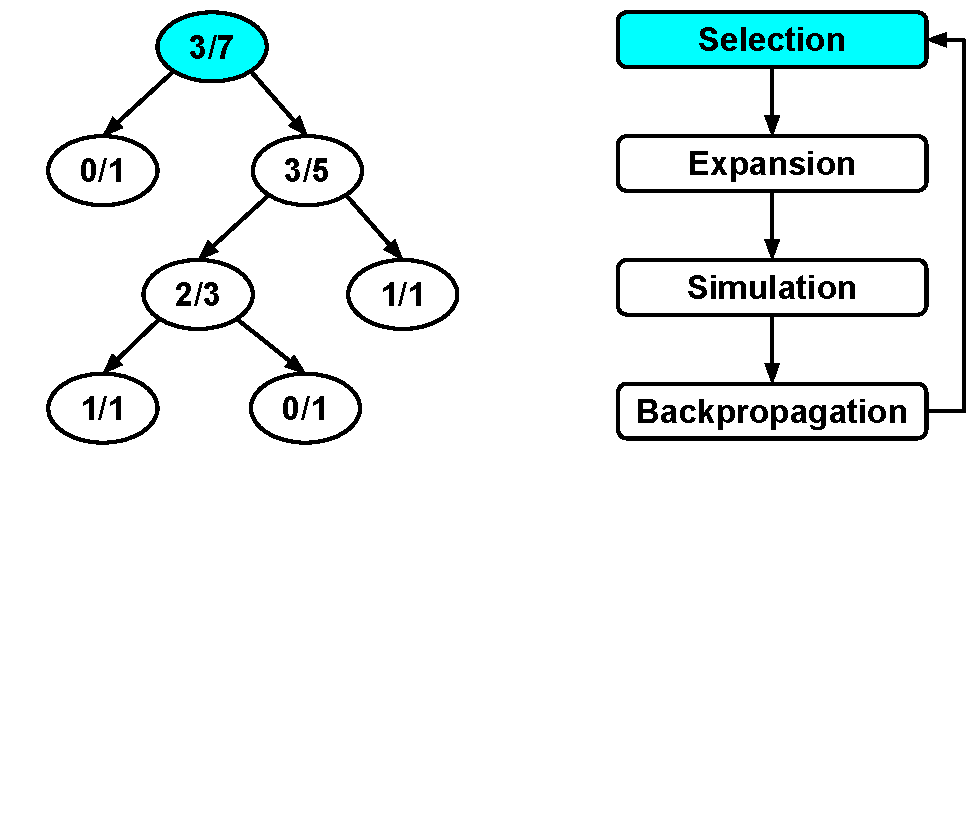
\includegraphics[width=6.5cm]{Diagrams/MCTSShort/MCTSShortTwoOneOne.pdf}
	\centering
\end{figure}
\end{frame}

\begin{frame}[fragile]
\frametitle{Four Steps Diagram}
\begin{figure}[h]
	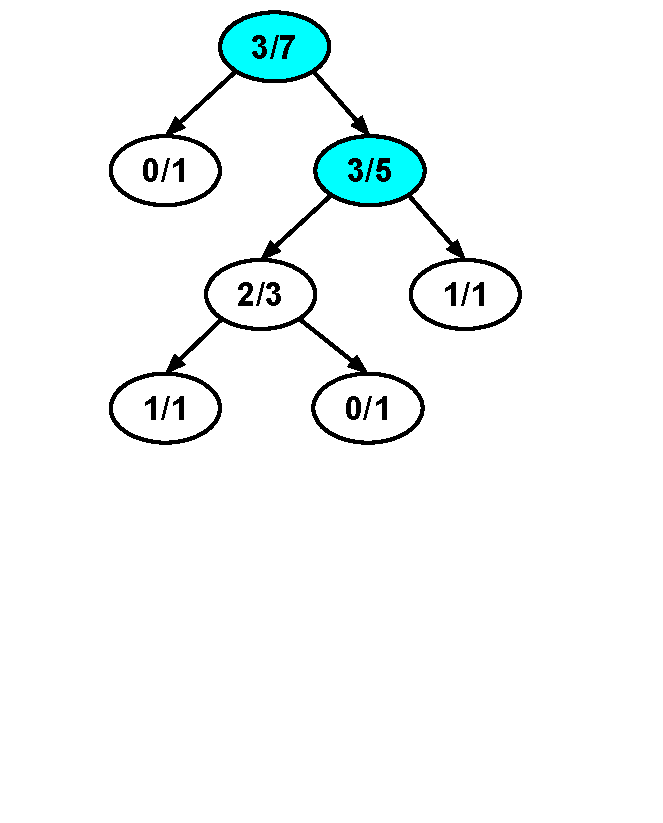
\includegraphics[width=6.5cm]{Diagrams/MCTSShort/MCTSShortTwoOneTwo.pdf}
	\centering
\end{figure}
\end{frame}

\begin{frame}[fragile]
\frametitle{Four Steps Diagram}
\begin{figure}[h]
	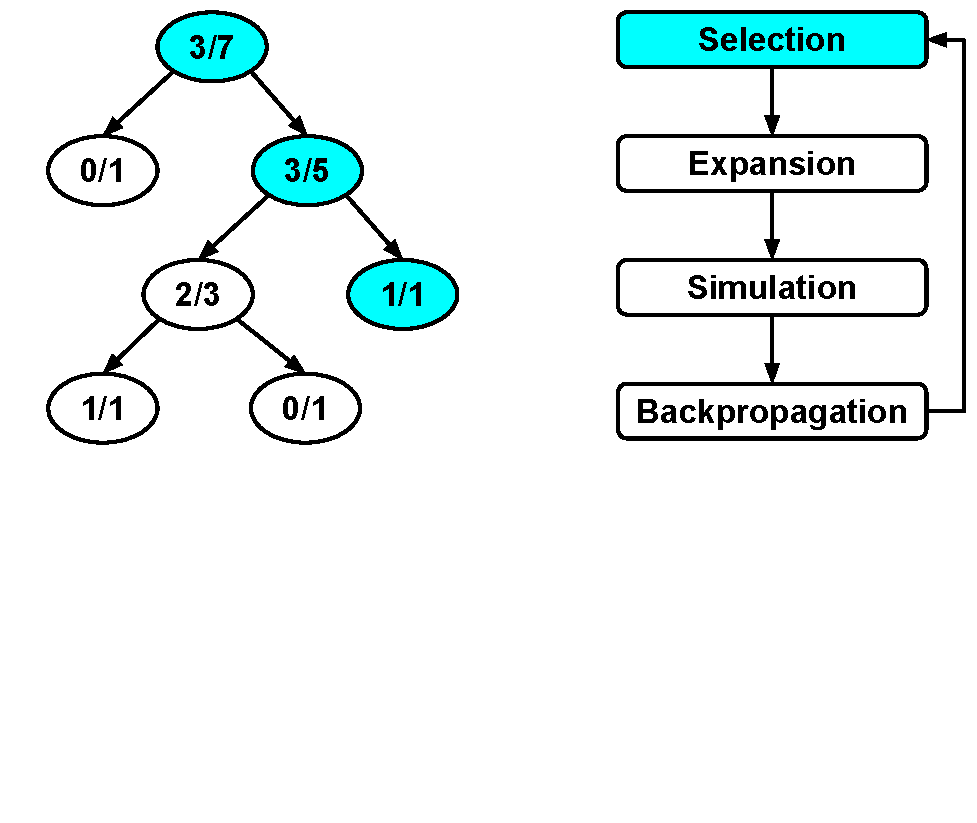
\includegraphics[width=6.5cm]{Diagrams/MCTSShort/MCTSShortTwoOneThree.pdf}
	\centering
\end{figure}
\end{frame}

\begin{frame}[fragile]
\frametitle{Four Steps Diagram}
\begin{figure}[h]
	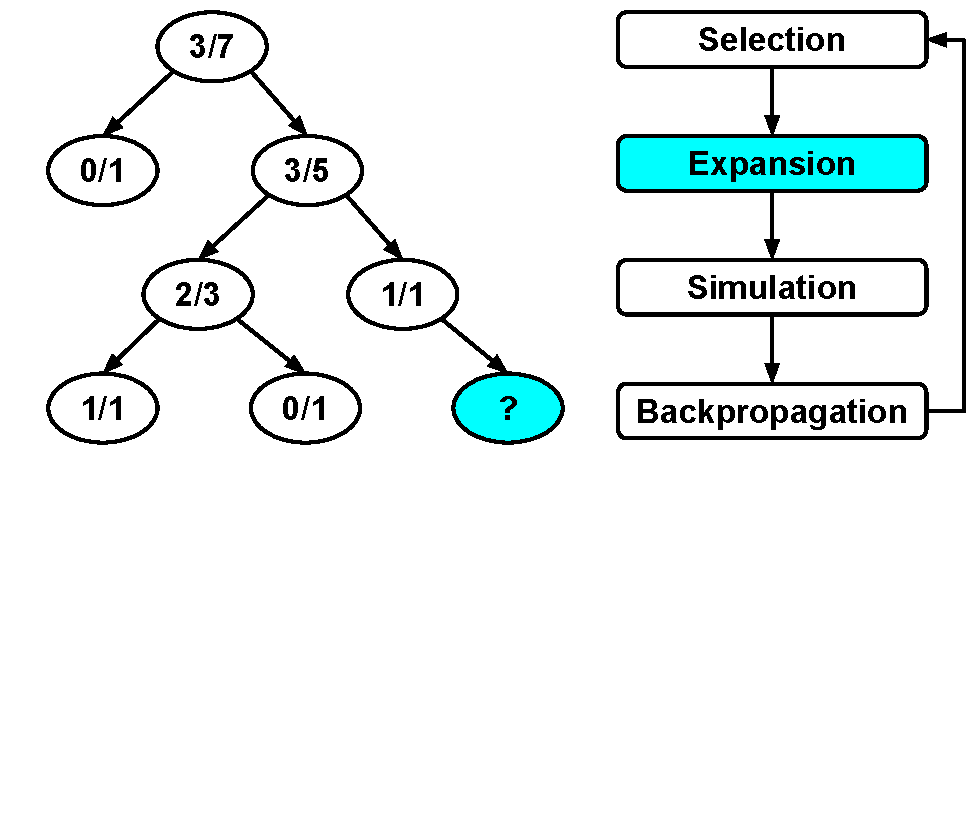
\includegraphics[width=6.5cm]{Diagrams/MCTSShort/MCTSShortTwoTwo.pdf}
	\centering
\end{figure}
\end{frame}

\begin{frame}[fragile]
\frametitle{Four Steps Diagram}
\begin{figure}[h]
	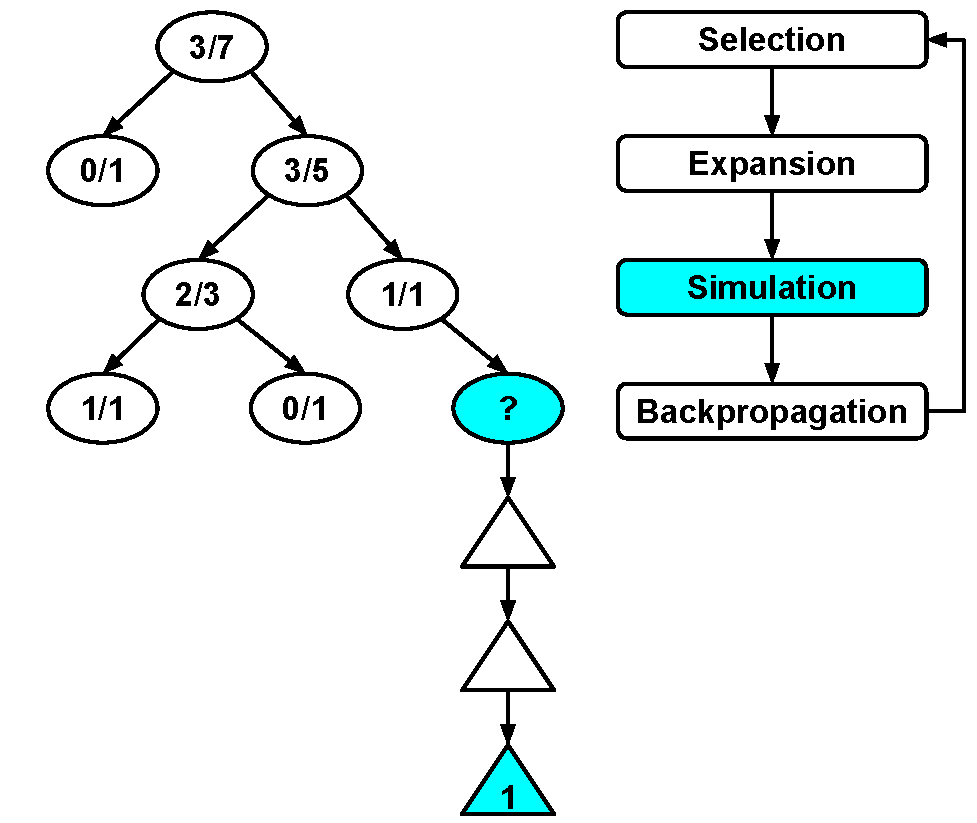
\includegraphics[width=6.5cm]{Diagrams/MCTSShort/MCTSShortTwoThree.pdf}
	\centering
\end{figure}
\end{frame}

\begin{frame}[fragile]
\frametitle{Four Steps Diagram}
\begin{figure}[h]
	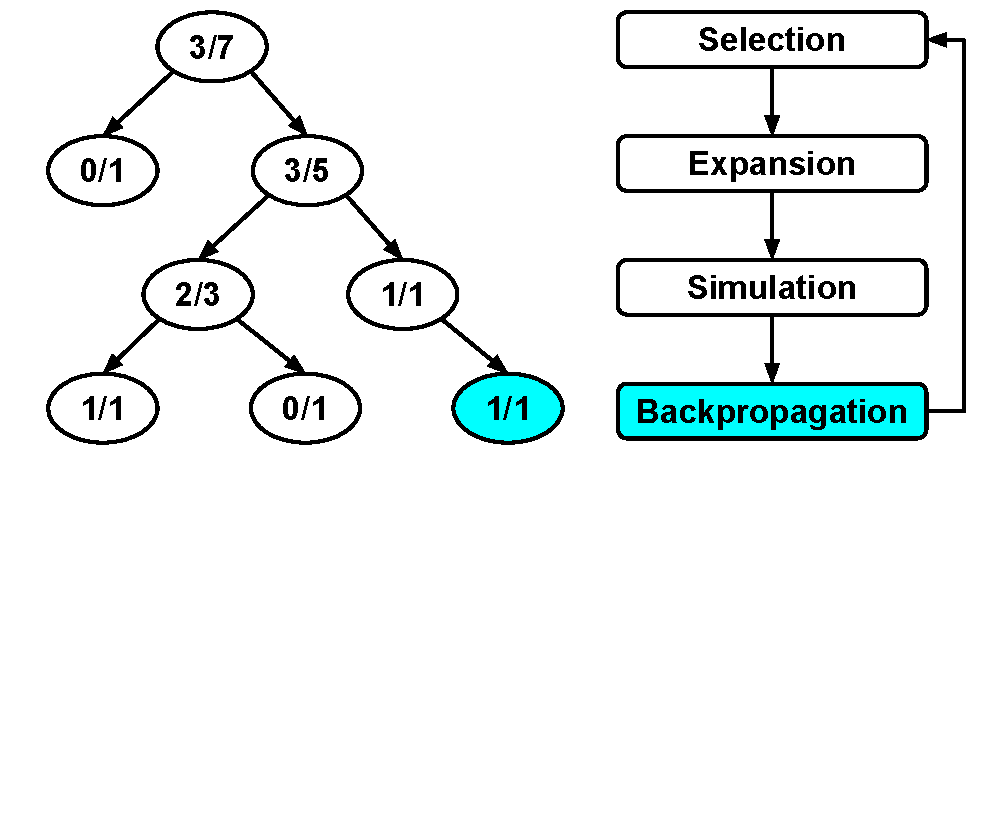
\includegraphics[width=6.5cm]{Diagrams/MCTSShort/MCTSShortTwoFourOne.pdf}
	\centering
\end{figure}
\end{frame}

\begin{frame}[fragile]
\frametitle{Four Steps Diagram}
\begin{figure}[h]
	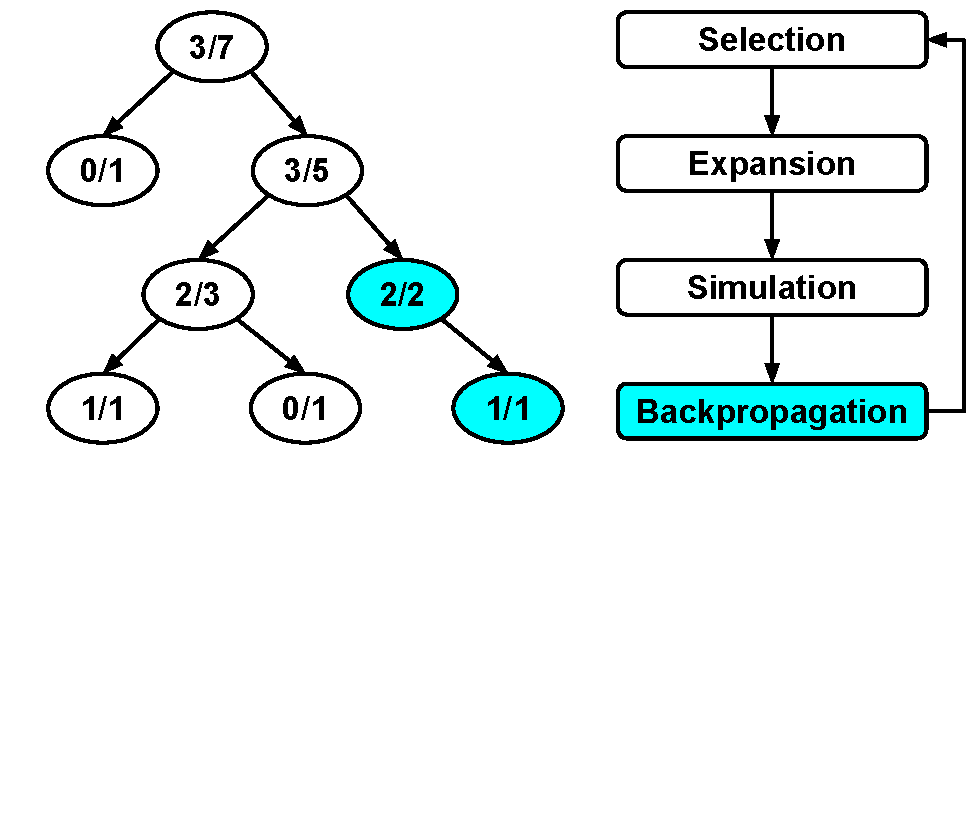
\includegraphics[width=6.5cm]{Diagrams/MCTSShort/MCTSShortTwoFourTwo.pdf}
	\centering
\end{figure}
\end{frame}

\begin{frame}[fragile]
\frametitle{Four Steps Diagram}
\begin{figure}[h]
	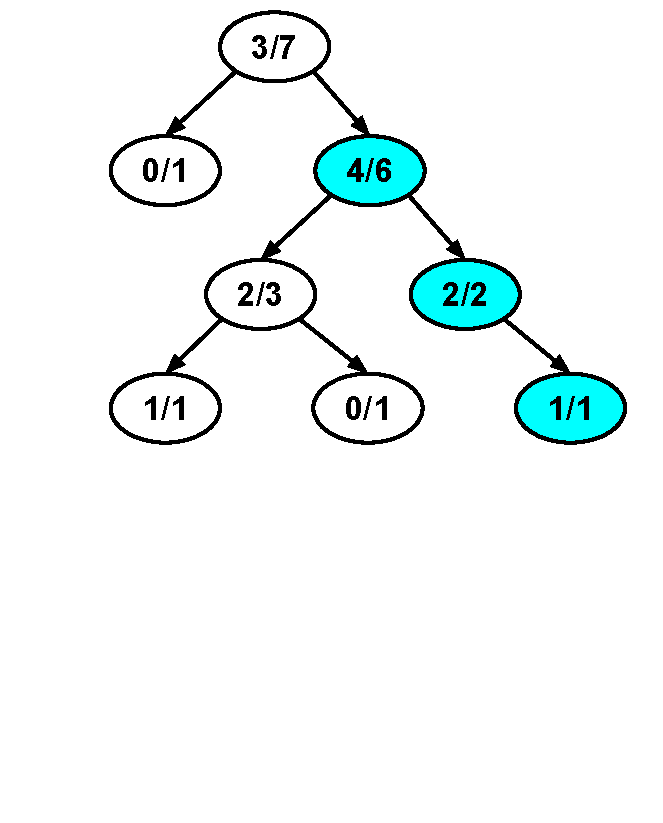
\includegraphics[width=6.5cm]{Diagrams/MCTSShort/MCTSShortTwoFourThree.pdf}
	\centering
\end{figure}
\end{frame}

\begin{frame}[fragile]
\frametitle{Four Steps Diagram}
\begin{figure}[h]
	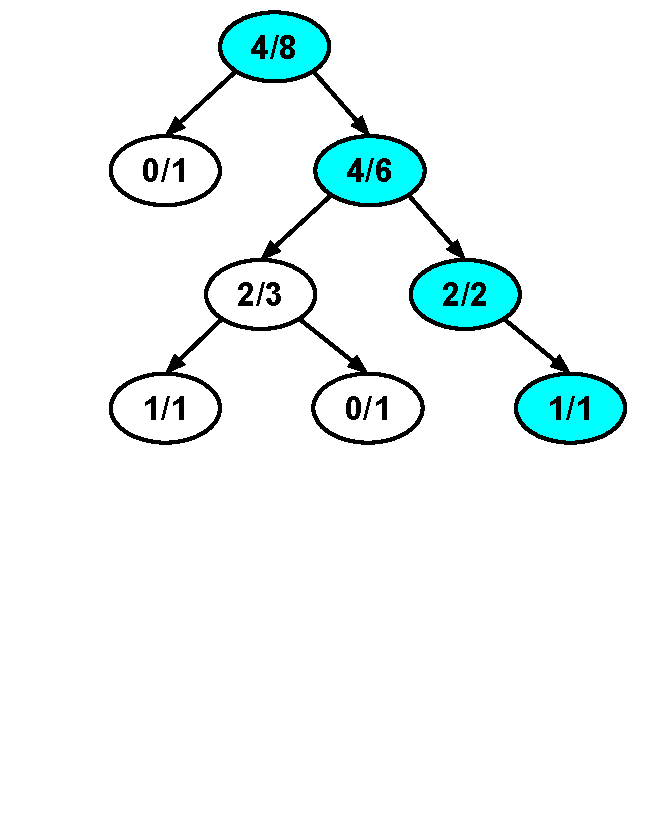
\includegraphics[width=6.5cm]{Diagrams/MCTSShort/MCTSShortTwoFourFour.pdf}
	\centering
\end{figure}
\end{frame}

%%%%%%%%%%%%%%%%%%%%%%%%%%Choosing move transition%%%%%%%%%%%%%%%%%%%%%%%%%%%%%

\begin{frame}
\frametitle{What Happens When We Choose a Move?}
Now we have:
\begin{itemize}
	\item{A tree structure}
	\item{A method of generating the tree}
\end{itemize}
What happens when we need to choose a move?
\end{frame}


\begin{frame}[fragile]
\frametitle{Choosing a Move}
\begin{figure}[h]
	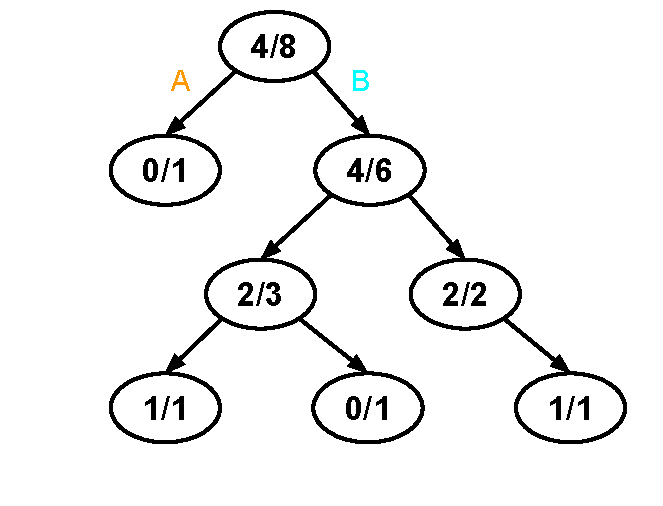
\includegraphics[width=6cm]{Diagrams/MakeAMove/MakeAMoveOne.pdf}
	\centering
\end{figure}
\end{frame}

\begin{frame}[fragile]
\frametitle{Choosing a Move}
\begin{figure}[h]
	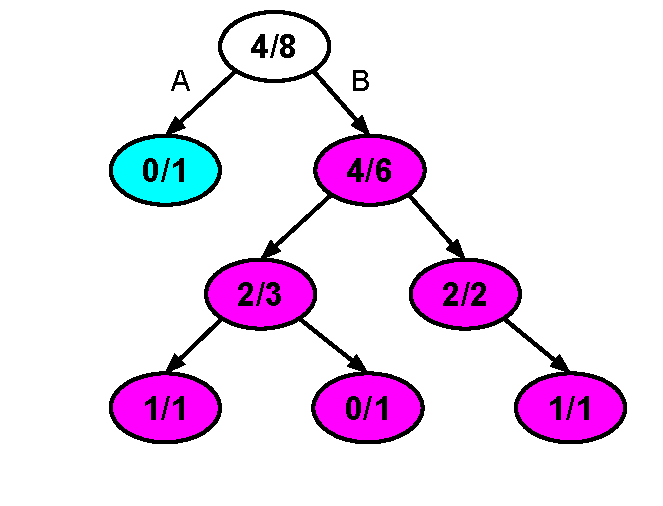
\includegraphics[width=6cm]{Diagrams/MakeAMove/MakeAMoveSubTrees.pdf}
	\centering
\end{figure}
\end{frame}

\begin{frame}[fragile]
\frametitle{Choosing a Move}
\begin{figure}[h]
	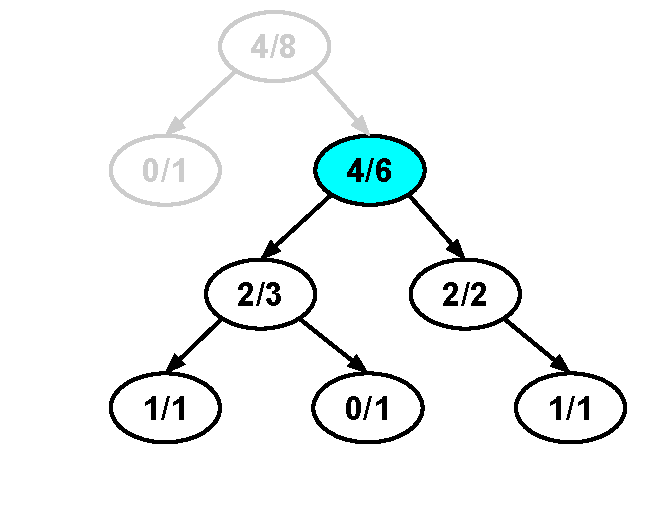
\includegraphics[width=6cm]{Diagrams/MakeAMove/MakeAMoveTwo.pdf}
	\centering
\end{figure}
\end{frame}

\begin{frame}[fragile]
\frametitle{Choosing a Move}
\begin{figure}[h]
	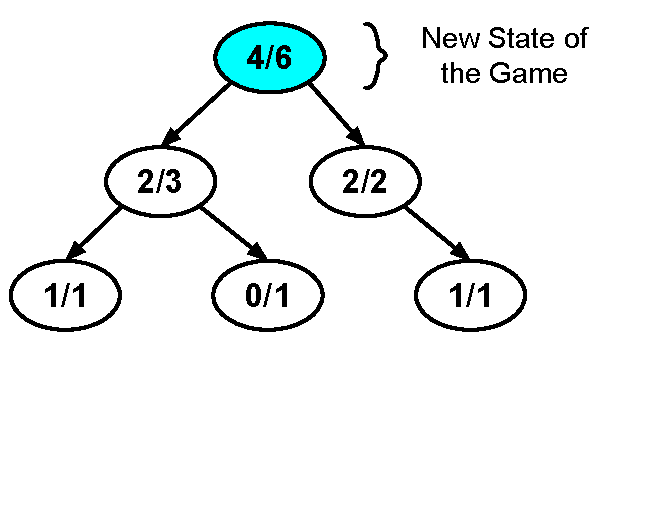
\includegraphics[width=6cm]{Diagrams/MakeAMove/MakeAMoveThree.pdf}
	\centering
\end{figure}
\end{frame}

\begin{frame}
\frametitle{Exploration vs Exploitation}
\begin{itemize}
	\item We might overlook better paths
	\item Exploration vs Exploitation
	\begin{itemize}
		\item Exploration looks at more options
		\item Exploitation focuses on the most promising path
	\end{itemize}
	\item Must find a balance between the two
\end{itemize}
\end{frame}

\begin{frame}[fragile]
\frametitle{Upper Confidence Bound Applied to Trees (UCT)}
\[
	UCT(node)
	{=}
	\alert{\underbrace{\color{black} \frac{W(node)}{N(node)}}_
		{{\text{Value of the Node}}}}
	{+}
	\alert{\underbrace{\color{black} \sqrt[C]{\frac{ln(N(parentNode))}{N(node)}}}_
		{\text{Exploration Bonus}}}
\]
\begin{itemize}
	\item W represents the number of simulated wins
	\item N represents the total number of simulations
	\item C is an experimental constant
	\item Used during tree traversal
	\item Balances exploration vs exploitation
\end{itemize}
\end{frame}

\section{Applying MCTS to Go}

\begin{frame}
\frametitle{Outline}
\tableofcontents[currentsection]
\end{frame}

\begin{frame}
\frametitle{MCTS applied to Go}
What variations can we make specific to Go? \\
In Go each player takes turn placing pieces on a game board
\begin{itemize}
	\item How much does the order of these moves matter?
	\item Can we use this to improve MCTS in the context of Go?
\end{itemize}
\end{frame}

\begin{frame}[fragile]
\frametitle{Tree Redundancy}
\begin{figure}[h]
	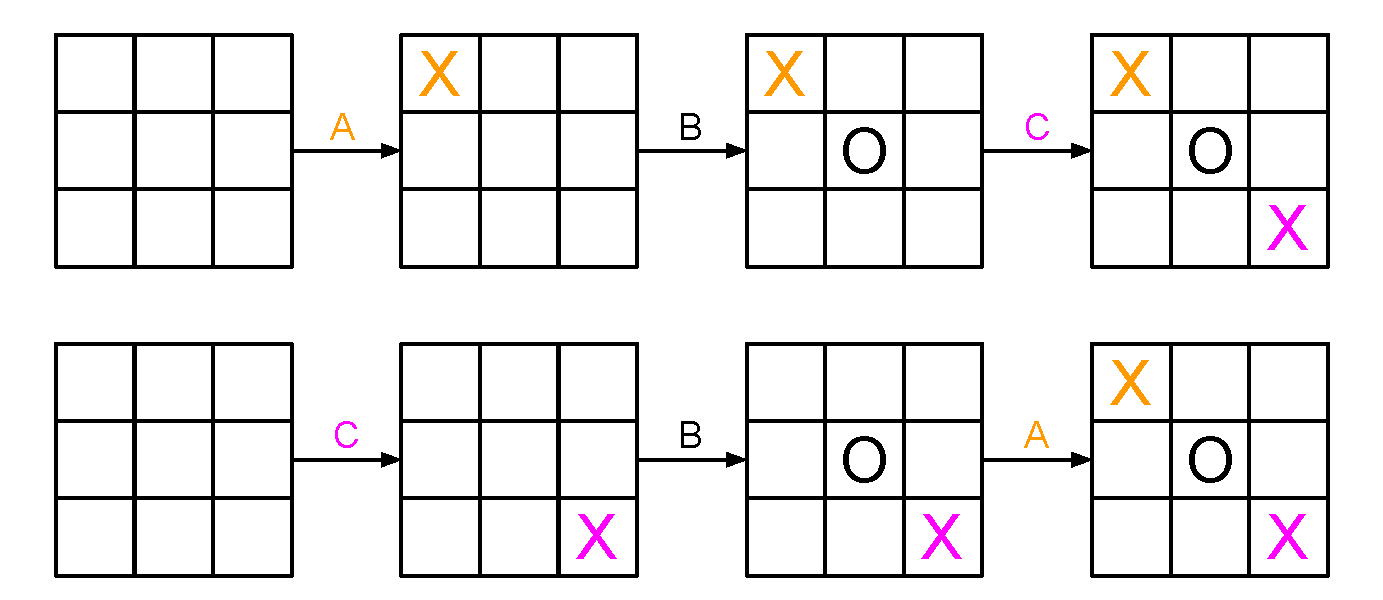
\includegraphics[width=11cm]{Diagrams/TicTacToe/MoveOrderNotMattering.pdf}
	\centering
\end{figure}
\end{frame}

\begin{frame}
\frametitle{Rapid Action Value Estimate (RAVE)}
\begin{itemize}
	\item Takes advantage of tree redundancy
	\item Stores the value of a move with in a subtree at each node
\end{itemize}
\end{frame}

\begin{frame}[fragile]
\frametitle{RAVE Diagram}
\begin{figure}[h]
	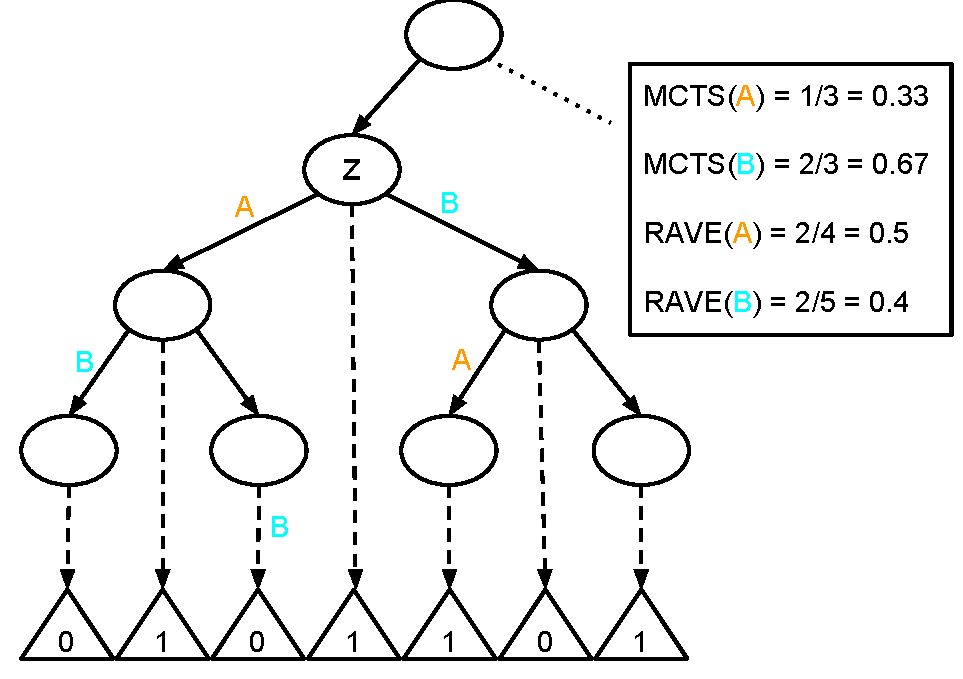
\includegraphics[width=8.5cm]{Diagrams/Rave/RAVEDiagram.pdf}
	\centering
\end{figure}
\end{frame}

\begin{frame}
\frametitle{RAVE}
\begin{itemize}
	\item Very powerful approach
	\item Each simulation provides us with more information
	\item This approach is used by the top computer Go programs
\end{itemize}
\end{frame}

\begin{frame}
\frametitle{Results}
\begin{itemize}
	\item Deterministic approaches could hardly defeat low level amateurs
	\item Computer Go programs use RAVE with MCTS
	\begin{itemize}
		\item MoGo
		\item Crazy Stone
	\end{itemize}
	\item Can compete against top pros in 9x9 Go
	\item Can compete against top pros in handicapped 19x19 Go
\end{itemize}
\end{frame}

\section{Applying MCTS to Narrative Generation}

\section{Conclusion} 

\end{document}


